
%% Copyright 2007-2020 Elsevier Ltd
%% 
%% This file is part of the 'Elsarticle Bundle'.
%% ---------------------------------------------
%% 
%% It may be distributed under the conditions of the LaTeX Project Public
%% License, either version 1.2 of this license or (at your option) any
%% later version.  The latest version of this license is in
%%    http://www.latex-project.org/lppl.txt
%% and version 1.2 or later is part of all distributions of LaTeX
%% version 1999/12/01 or later.
%% 
%% The list of all files belonging to the 'Elsarticle Bundle' is
%% given in the file `manifest.txt'.
%% 

%% Template article for Elsevier's document class `elsarticle'
%% with numbered style bibliographic references
%% SP 2008/03/01
%%
%% 
%%
%% $Id: elsarticle-template-num.tex 190 2020-11-23 11:12:32Z rishi $
%%
%%
%\documentclass[preprint,12pt]{elsarticle}

%% Use the option review to obtain double line spacing
%% \documentclass[authoryear,preprint,review,12pt]{elsarticle}

%% Use the options 1p,twocolumn; 3p; 3p,twocolumn; 5p; or 5p,twocolumn
%% for a journal layout:
%% \documentclass[final,1p,times]{elsarticle}
%% \documentclass[final,1p,times,twocolumn]{elsarticle}
\documentclass[final,3p,times,review]{elsarticle}
%% \documentclass[final,3p,times,twocolumn]{elsarticle}
%% \documentclass[final,5p,times]{elsarticle}
%% \documentclass[final,5p,times,twocolumn]{elsarticle}

%% For including figures, graphicx.sty has been loaded in
%% elsarticle.cls. If you prefer to use the old commands
%% please give \usepackage{epsfig}

%% The amssymb package provides various useful mathematical symbols
\usepackage{amssymb}
\usepackage{amsmath}
\usepackage{float}
%\usepackage{url}
%\usepackage{hyperref}

\usepackage{graphicx}  % For including figures

\usepackage[utf8]{inputenc}
\usepackage[T1]{fontenc}
\usepackage{lmodern}
\usepackage{booktabs}
%\usepackage{graphicx}
\usepackage[figurename=Fig.,labelfont=bf,labelsep=period]{caption}
\usepackage{subcaption}
\usepackage{lineno}
\usepackage{natbib}
%\usepackage{gensymb}
\usepackage{listings}
\usepackage[ruled,vlined]{algorithm2e}
%\usepackage{amsfonts} % for dummy text
%% The amsthm package provides extended theorem environments
%% \usepackage{amsthm}
\usepackage{adjustbox} % for wide tables to fit page width
\usepackage{tabularx}   % smart column wrapping to avoid scaling
\usepackage{array}      % better column defs
\usepackage{makecell}   % easy multi-line headers (optional)
\usepackage[dvipsnames]{xcolor}
\newcolumntype{Y}{>{\raggedright\arraybackslash}X} % flexible, left-aligned column


%% The lineno packages adds line numbers. Start line numbering with
%% \begin{linenumbers}, end it with \end{linenumbers}. Or switch it on
%% for the whole article with \linenumbers.
%% \usepackage{lineno}
\usepackage{ulem} % for \sout command
\journal{Building and Environment}

\begin{document}

\begin{frontmatter}

%% Title, authors and addresses

%% use the tnoteref command within \title for footnotes;
%% use the tnotetext command for theassociated footnote;
%% use the fnref command within \author or \address for footnotes;
%% use the fntext command for theassociated footnote;
%% use the corref command within \author for corresponding author footnotes;
%% use the cortext command for theassociated footnote;
%% use the ead command for the email address,
%% and the form \ead[url] for the home page:
%% \title{Title\tnoteref{label1}}
%% \tnotetext[label1]{}
%% \author{Name\corref{cor1}\fnref{label2}}
%% \ead{email address}
%% \ead[url]{home page}
%% \fntext[label2]{}
%% \affiliation{organization={},
%%             addressline={},
%%             city={},
%%             postcode={},
%%             state={},
%%             country={}}
%% \fntext[label3]{}

\title{Visual Privacy Assessment in Urban Design through BIM and Fuzzy Logic}

%% use optional labels to link authors explicitly to addresses:
%% \author[label1,label2]{}
%% \affiliation[label1]{organization={},
%%             addressline={},
%%             city={},
%%             postcode={},
%%             state={},
%%             country={}}
%%
%% \affiliation[label2]{organization={},
%%             addressline={},
%%             city={},
%%             postcode={},
%%             state={},
%%             country={}}

\author[1]{Naimeh Sadeghi}\corref{cor1}

\author[1]{Sepehr Jahantab}

\affiliation[1]
{
    organization={Faculty of Civil Engineering, K.N. Toosi University of Technology},
    city={Tehran},
    postcode={19967-15433},
    country={Iran}}
\cortext[cor1]{Corresponding author: sadeghi@kntu.ac.ir}

\begin{abstract}
As cities continue to urbanize and populations grow denser, the challenge of balancing privacy with view quality in architectural design has become increasingly critical. Existing methods for privacy assessment often fail to account for the unique spatial layouts of buildings or the subjective perceptions of occupants. This paper proposes a novel framework that addresses these gaps by integrating visibility analysis with Building Information Modeling (BIM) to quantify privacy in buildings. The framework combines grid-based visibility maps with fuzzy membership functions to assess both physical factors—such as distance and angle—and subjective user perceptions of privacy. BIM-based 3D analysis simulates visibility across various points within a building, generating privacy indices that reflect the unique spatial configurations of each structure. The methodology is validated through experiments, demonstrating how design elements, including window size and room layout, significantly impact privacy. This data-driven approach empowers architects and urban designers to make informed decisions that consider occupant privacy alongside other functional design goals. While this research addresses a significant gap, future work may explore integrating culturally specific membership functions, optimization algorithms for space planning, and expanding the framework to evaluate additional architectural parameters such as view quality and occupant comfort.

\end{abstract}

\begin{keyword}
%% keywords here, in the form: keyword \sep keyword
visibility analysis \sep privacy mapping \sep sustainable design \sep spatial layout \sep subjective perception
\end{keyword}

\end{frontmatter}

%% \linenumbers
\section{Introduction}
In recent decades, the concept of sustainable development has gained widespread attention due to its critical role in shaping the present and future quality of human life \cite{hariram2023}. Sustainable development is traditionally defined through three interconnected pillars: environmental, economic, and social dimensions. Achieving sustainability requires a balance among these aspects, ensuring that development meets current needs without compromising the ability of future generations to meet their own \cite{mensah2019}.

The construction industry, as one of the world's largest and most influential sectors, has primarily concentrated on the environmental aspects of sustainability \cite{lima2021}. This focus is evident in research addressing waste management \cite{negash2021}, energy efficiency \cite{mousavi2023}, water conservation\cite{arman2021}, material recycling, and pollution reduction throughout the construction life-cycle. However, the social dimension of sustainability—particularly its impact on human well-being—has not received equal attention \cite{debrah2022}.

A critical aspect of social sustainability in the built environment is residents’ comfort, defined as the state of mind where occupants are satisfied with the internal and external conditions of their living spaces \cite{yildiz2020}. This comfort is evaluated across four main metrics: thermal, visual, acoustic, and respiratory comfort, each contributing to the occupants' health and productivity \cite{faraji2023}. Among these, visual comfort plays a crucial role, encompassing elements like adequate natural lighting, visual privacy, and the quality of views both inside and outside the building \cite{abd2023}.

The focus of this research is on visual privacy, an essential yet frequently overlooked component of visual comfort, particularly in environments where cultural norms and social expectations place a high value on personal space and seclusion. Visual privacy refers to the degree to which individuals feel shielded from unwanted observation while performing everyday activities \cite{lis2021}. This aspect of comfort is crucial in ensuring psychological well-being and fostering a sense of security, as it allows occupants to maintain control over their visual exposure to the outside world \cite{ mansor2020}. 

One of the critical implications of visual privacy is its influence on the use of elements such as curtains or blinds \cite{elgadra2023}. These solutions, while essential for maintaining privacy, directly impact the availability of natural light and views, which are integral to creating comfortable and energy-efficient spaces. Natural light not only enhances visual comfort but also reduces energy use by lowering reliance on artificial lighting \cite{gago2015}. However, balancing privacy with daylight access is frequently neglected in design. Furthermore, quantifying visual privacy enables the development of models that optimize layouts, addressing both environmental efficiency and comfort \cite{elbatran2021,bahdad2021,khani2022,lotfabadi2023}.

Visual privacy is an essential aspect of building design, directly influencing occupants' comfort\cite{ day2020}. Visual privacy is particularly relevant in settings such as, residential buildings, and healthcare facilities, where the need for natural light and visibility must be carefully managed to prevent unwanted exposure or feelings of vulnerability \cite{kwong2020, peng2024}.

In culturally sensitive contexts, quantifying visual privacy is inherently complex and subjective \cite{kent2020}. Different societies have distinct thresholds for acceptable visibility, which significantly influence building design. To address the subjective nature of privacy feeling, we employ fuzzy logic, which extends beyond traditional visibility analyses by incorporating variables such as distance, viewing angles, and occupants' perceived exposure \cite{kim2013}. Fuzzy logic provides a mean to quantify human perception and subjective judgments \cite{zadeh1996,shepard2005,zadeh2015}. This flexible approach allows context-specific privacy assessments to based on individual or cultural needs.

To evaluate visual privacy at a micro-level, integrating detailed building and environmental data is crucial. Building Information Modeling (BIM) provides a comprehensive digital representation of physical structures, capturing architectural elements, spatial configurations, and environmental conditions \cite{liu2015,lu2017, chong2017,llatas2020,olanrewaju2022}. This makes BIM an indispensable tool for simulating and analyzing privacy, offering insights often missed in traditional methods.

By integrating BIM with fuzzy logic, this study establishes a privacy quantification framework that merges real-world viewing conditions with human perception and subjective experience. This approach provides deeper insights into how design choices influence occupants' sense of privacy. It equips architects and design algorithms with a powerful tool to incorporate privacy as a key factor in optimizing building layouts, striking a balance between comfort and functionality across varied cultural and spatial contexts.

\paragraph{Contributions.}
This paper advances visual-privacy analysis beyond façade exposure by focusing on \textit{interior, BIM-aware} mapping. Our contributions are:
(i) a multi-height, grid-based 3D ray-casting scheme inside rooms with explicit \emph{window-through-window} checks;
(ii) a perception layer using user-tunable fuzzy membership functions for distance and angle (with default parameters) and a soft-max aggregation that interpolates between mean and max;
(iii) clarified implementation constraints for correctness (storey-constrained rays, termination at opaque elements); and
(iv) evidence of computational scalability through runtime/scale reporting on multi-room/multi-building cases.

\section{Literature Review}

To explore this topic, this section reviews the relevant literature on two interconnected aspects. The first focuses on visibility analysis approaches, which form the foundation for understanding visual conditions within a space, including factors such as view access and spatial openness. The second explains methods for evaluating visual privacy in buildings.

\subsection{Visibility Analysis Approaches}
Visibility analysis is a critical component of understanding how spatial design influences occupants' interactions with their environment \cite{askarizad2020}. It involves assessing the extent to which spaces are visually accessible, and plays a key role in optimizing the balance between openness and privacy in building design \cite{inglis2022}.

One of the primary tools in visibility analysis is isovist analysis. Isovists represent the visible area from a specific point within a space, offering insights into how much of the surrounding environment is within view. This approach is particularly useful for evaluating spatial openness, identifying visual obstructions, and determining potential sightlines. By analyzing isovists, designers can better understand how visibility changes based on spatial layout and occupant positioning. An isovist field is a spatial analysis technique that involves generating isovists from many points throughout a space, which together create a field that can show variations in visibility across that space \cite{ benedikt1979,turner2001, hosseini2022}.

Another widely used method is viewshed analysis. Viewsheds identify the areas that are visible from a particular vantage point, typically accounting for environmental features such as terrain, buildings, and vegetation\cite{inglis2022}. This technique is commonly used in urban planning and landscape architecture to assess the visual impact of proposed developments and optimize sightlines for aesthetic or functional purposes \cite{misthos2019, gillings2020,stein2022}. Both isovist and viewshed involve casting rays to determine visible regions, but they are used in different contexts and at different scales. Essentially, both show what is visible from a point or set of points\cite{cavaglia2024}.

Building on traditional viewshed analysis, fuzzy viewsheds incorporate uncertainty and subjectivity into visibility assessments \cite{fisher1992, fisher1994, alberti2017, cimburova2022}. Unlike conventional binary viewsheds, which classify areas as either visible or not, fuzzy viewsheds assign a degree of visibility to each point in the environment. This reflects the varying levels of clarity or obstruction that can influence perception. For instance, factors like distance, viewing angle, and environmental context affect how clearly an observer perceives a space. This approach captures the gradual transition between fully visible and non-visible areas, reflecting the subjective nature of human perception. At the heart of this method are fuzzy membership functions, which define how factors such as angle and distance influence perceived visibility. These functions map each input---such as the distance from an observer or the angle of view---to a value between 0 and 1, representing the degree to which a given point is considered "visible" \cite{fisher2024}.


In addition to these methods, view access and quality assessments evaluate the extent and quality of views from key locations within a building \cite{biljecki2021}. Metrics such as the percentage of visible outdoor space or the clarity of sightlines are used to determine how well a design meets occupants' needs. View quality assessments often consider factors like framing, depth of field, and the diversity of visible elements \cite{kent2020,abdelrahman2023}.

More advanced visibility analysis approaches, such as three-dimensional (3D) visibility models, provide a deeper understanding of visual conditions by incorporating vertical dimensions and complex geometries \cite{morello2009, suleiman2013,chen2021,krukar2021, parent2023}. These models extend traditional 2D methods, including isovists and viewsheds, into 3D space. Beyond extending these traditional methods, 3D models often integrate dynamic elements such as lighting and occupant movement, simulating real-world visibility scenarios \cite{othman2019, snopkova2023}. Advanced computational tools like Rhino with Grasshopper or GIS platforms enable real-time, interactive visibility analysis, allowing designers to optimize layouts based on visibility and view quality metrices \cite{wu2023, khaleel2023, guo2023}.

\subsection{Visual Privacy}
The concept of visual privacy is inherently subjective, varying significantly based on individual experiences and cultural backgrounds. For instance, Al-Kodmany highlights a pronounced gender disparity in privacy needs, demonstrating that visual privacy is of greater importance for women in Damascus, Syria, than for men\cite{Kodmany1999}. Similarly, Rahim explores differences in privacy expectations between Muslims and Malaysians, emphasizing how Islamic architectural traditions often prioritize gender-segregated spaces—a feature less emphasized in Malaysian design \cite{rahim2015}. 

Several studies have assessed visual privacy using questionnaire-based methods, offering valuable insights into individuals' privacy perceptions within various architectural settings. For example, some studies examined employee experiences in a LEED-certified building where visual privacy was one of the key consideration, highlighting the balance between environmental performance and occupants’ privacy needs \cite{Altomonte2013,Schiavon2014,Guo2021}. 

Building separation standards vary worldwide to balance privacy, access to natural light, and urban density. In the UK, cities like London and Manchester recommend 18-21 meters between residential buildings\cite{ LondonGuidelines, ManchesterGuidelines}. Australia’s guidelines depend on height, ranging from 12 to 24 meters\cite{NSWApartmentDesign}. In Canada, Toronto requires at least 25 meters between tall buildings for light and privacy \cite{TorontoTallBuildings}. In the U.S., cities like New York and Chicago focus on setbacks and zoning laws rather than fixed distances. These standards reflect local priorities, with denser cities often relying on design solutions to ensure livability \cite{ NYCZoning}.

Despite these efforts, research quantifying the visual privacy of buildings remains limited. Moreover, the few studies that exist predominantly focus on the building envelope, often overlooking the crucial role of interior layouts. For example, Al-Khalili et al. investigated the effects of visual angle and brightness ratio on perceived privacy, using linear regression to model privacy levels based on window visibility and brightness factors \cite{alkhalili2018}. However, their approach focuses mainly on external features, neglecting internal spatial dynamics.

Similarly, zheng et al.\cite{zheng2021} proposed the Potential Visual Exposure Index (PVEI) to quantify visual privacy in buildings, considering factors like window size and spacing, as well as the horizontal and vertical angles of observers relative to occupants. Yet, this method does not account for floor plans or the subjective experiences of individuals, highlighting the need for more comprehensive evaluation approaches. 

\subsection{Visibility \& privacy in context: from VE/VO and Spatial Openness to (I-)PVEI and this work}
A long-standing line of research connects form, density and privacy, noting that perceived crowding and visual intrusion increase with built density even when objective measures are similar \citep{Churchman1999}. Within visibility-centric methods, two early strands are especially relevant. The first develops \textit{Visual Exposure} (VE), which quantifies inter-façade penetration, and \textit{Visual Openness} (VO), which captures perceived openness in urban morphologies \citep{ShachPinsly2007,ShachPinsly2011}. A parallel strand formalizes \textit{Spatial Openness} and related 3D visibility constructs, linking quantitative visibility to perceived density and visual experience in compact dwellings \citep{FisherGewirtzman2003a,FisherGewirtzman2003b,FisherGewirtzman2017,FisherGewirtzman2018}.

More recent work proposes the \textit{Potential Visual Exposure Index} (PVEI) for residential privacy risk at façades, with emphasis on surrounding observer fields; follow-on studies (often termed I-PVEI) refine directionality/weighting to improve discrimination at openings \citep{zheng2021,Zheng2023_IPVEI}. Comprehensive reviews on view/visibility metrics further situate these indices within broader building-performance and view-quality debates \citep{AbdAlhamid2023Review}.

\paragraph{How this study differs.}
Compared with VE/VO and Spatial Openness (largely exterior/morphological) and PVEI/I-PVEI (façade/opening-oriented), we quantify \emph{interior} privacy using a BIM-aware, multi-height vantage grid, enforce storey-constrained rays with opaque-surface termination and explicit window-through-window rules, and incorporate a \emph{perception layer} (fuzzy membership functions for distance/angle) aggregated with a soft-max operator. This design produces spatial privacy maps and indices suitable for design iteration at room scale while remaining computationally tractable.

\begin{table}[H]
\centering
\caption{Compact summary of related visibility/visual-privacy methods.}
\label{tab:prior_comparison}
\setlength{\tabcolsep}{4pt}
\renewcommand{\arraystretch}{1.15}
{\sloppy
\begin{tabularx}{\textwidth}{@{}p{3.3cm} p{2.4cm} Y p{2.0cm} Y Y@{}}
\toprule
\textbf{Method} & \textbf{Scale} & \textbf{Inputs} & \textbf{Interiors} & \textbf{Kernel} & \textbf{Outputs} \\
\midrule
VE \citep{ShachPinsly2007} &
Block/façade &
Façade geometry; inter-window &
No &
Line-of-sight counts &
Exposure ranking \\

VO \citep{ShachPinsly2011} &
Block/neigh. &
Urban form; open-space &
No (exterior) &
Openness metrics &
Openness index; comparison \\

\makecell[l]{Spatial Openness (SOI)\\\citep{FisherGewirtzman2003a,FisherGewirtzman2003b}} &
Unit/block &
3D geometry; view volumes &
Partial (limited) &
3D visibility volumes &
SOI; density link \\

\makecell[l]{Weighted views\\\citep{FisherGewirtzman2018}} &
Unit/block &
3D geometry; weighted targets &
Partial &
Viewshed + weights &
Weighted-view index \\

\makecell[l]{PVEI\\\citep{zheng2021}} &
Façade/opening &
Context; observer fields &
No (façade) &
Visual-incursion tally &
Opening privacy risk \\

\makecell[l]{I-PVEI\\\citep{Zheng2023_IPVEI}} &
Façade/opening &
+ direction weighting &
No &
PVEI + dir. weights &
Improved façade privacy \\

\textbf{This work} &
\textbf{Room/interior} &
\textbf{BIM model; multi-height grid; window-through-window rule} &
\textbf{Yes (explicit)} &
3D ray-casting; opaque stop &
Interior privacy maps; PI/SPI \\
\bottomrule
\end{tabularx}
\fussy
}
\end{table}

\section{Problem Statement}
The growing importance of visual privacy in architectural design is particularly evident in the context of urban density and open-plan layouts. However, despite the widespread availability of ray-casting approaches, including visibility analysis tools such as isovists and viewsheds, these methods remain underutilized in privacy quantification. These methods are primarily employed for optimizing visibility, improving spatial accessibility, and urban planning, leaving their potential for systematic privacy evaluation within architectural design largely untapped. A more comprehensive approach is needed to harness these tools for assessing and enhancing privacy in both exterior and interior environments.

Most existing studies on visual privacy focus on external factors such as window placement, building orientation, and external obstructions. However, they often fail to account for cultural and individual variability, limiting their applicability across diverse contexts. This oversight results in assessments that inadequately capture the subjective and culturally sensitive aspects of privacy and comfort. Additionally, the critical role of interior spatial configurations is frequently overlooked in existing research. 

BIM offers a promising solution to these challenges by enabling the simulation of visibility and privacy metrics within detailed digital models. This allows designers to test and refine strategies that balance visibility and privacy. While BIM is widely recognized for its contributions to energy efficiency and material optimization, its potential to advance social sustainability—particularly in enhancing visual privacy and comfort—remains under-explored.

Fuzzy logic also shows potential in addressing subjective aspects of privacy. However, current approaches often rely on simplified mathematical models, such as distance decay (1/d²) or cosine of the view angle, to define fuzzy membership functions for visual assessment. These generalized methods fail to capture the human perception, shaped by cultural norms, social contexts, and individual preferences.

To bridge these gaps, this study proposes a novel framework that integrates ray-casting techniques with fuzzy logic to quantify visual privacy. Leveraging BIM, the framework incorporates both exterior and interior spatial configurations to provide a holistic privacy assessment. By incorporating user-centric fuzzy logic models, this approach enables the systematic evaluation of subjective privacy perceptions, offering designers insights to optimize privacy in various architectural contexts.

\section{Methodology}
Our pipeline (Fig.~\ref{fig:pipeline}) comprises five stages:
(i) BIM preprocessing, (ii) grid generation, (iii) ray casting,
(iv) ray scoring, and (v) space-level aggregation.

\begin{figure}[H]
    \centering
    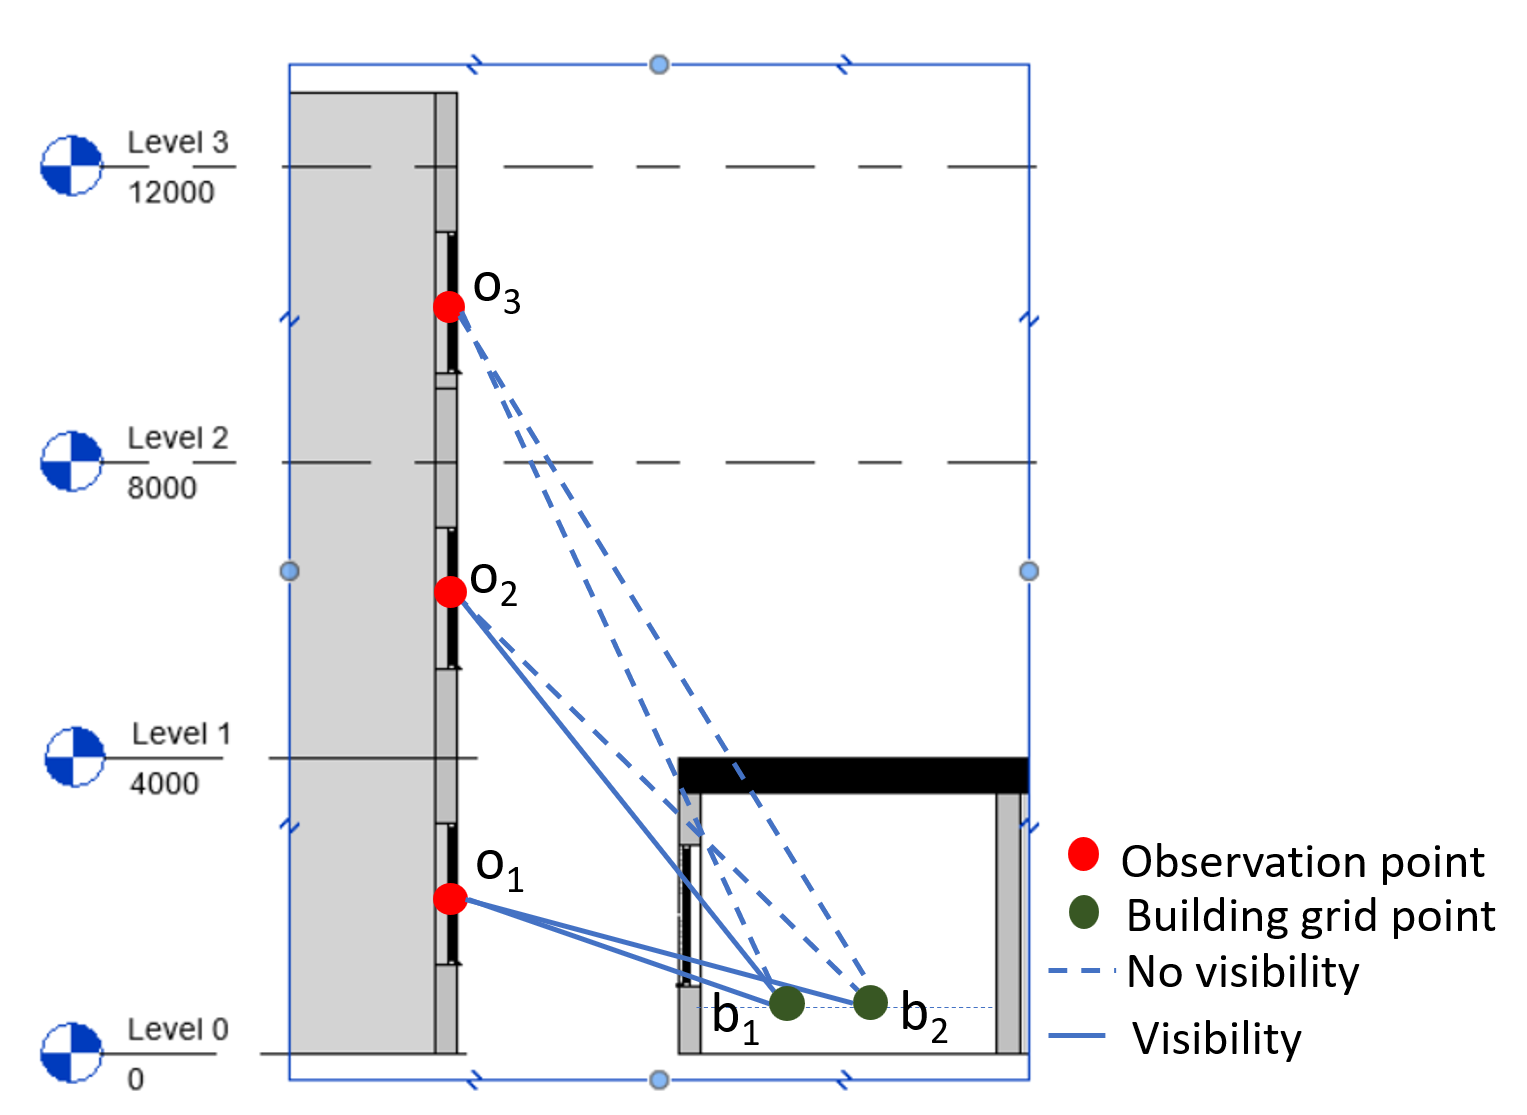
\includegraphics[width=0.8\linewidth]{visibility.png}
    \caption{Processing pipeline from BIM preprocessing to space-level privacy aggregation.}
    \label{fig:pipeline}
\end{figure}

\subsection{BIM Model Setup}
We assume valid, watertight BIM geometry with explicit wall, slab, and window semantics. Models use a right-handed, $z$-up coordinate frame in metres. Window panes are treated as transparent surfaces bounded by opaque frames, and all other elements are opaque occluders. Neighboring context follows the same conventions.

Given a BIM model with interior layout (rooms, partitions, windows) and surrounding context (neighboring buildings and façades), two illustrative examples are shown in Fig.~\ref{fig:bim_models}. The first case (a) places two buildings with facing windows, creating direct lines of sight; the second (b) introduces a third building with a window facing the leftmost building, increasing exposure. Models were created with OBIM (Three.js based), but the approach is platform-agnostic.

\begin{figure}[ht!]
    \centering
    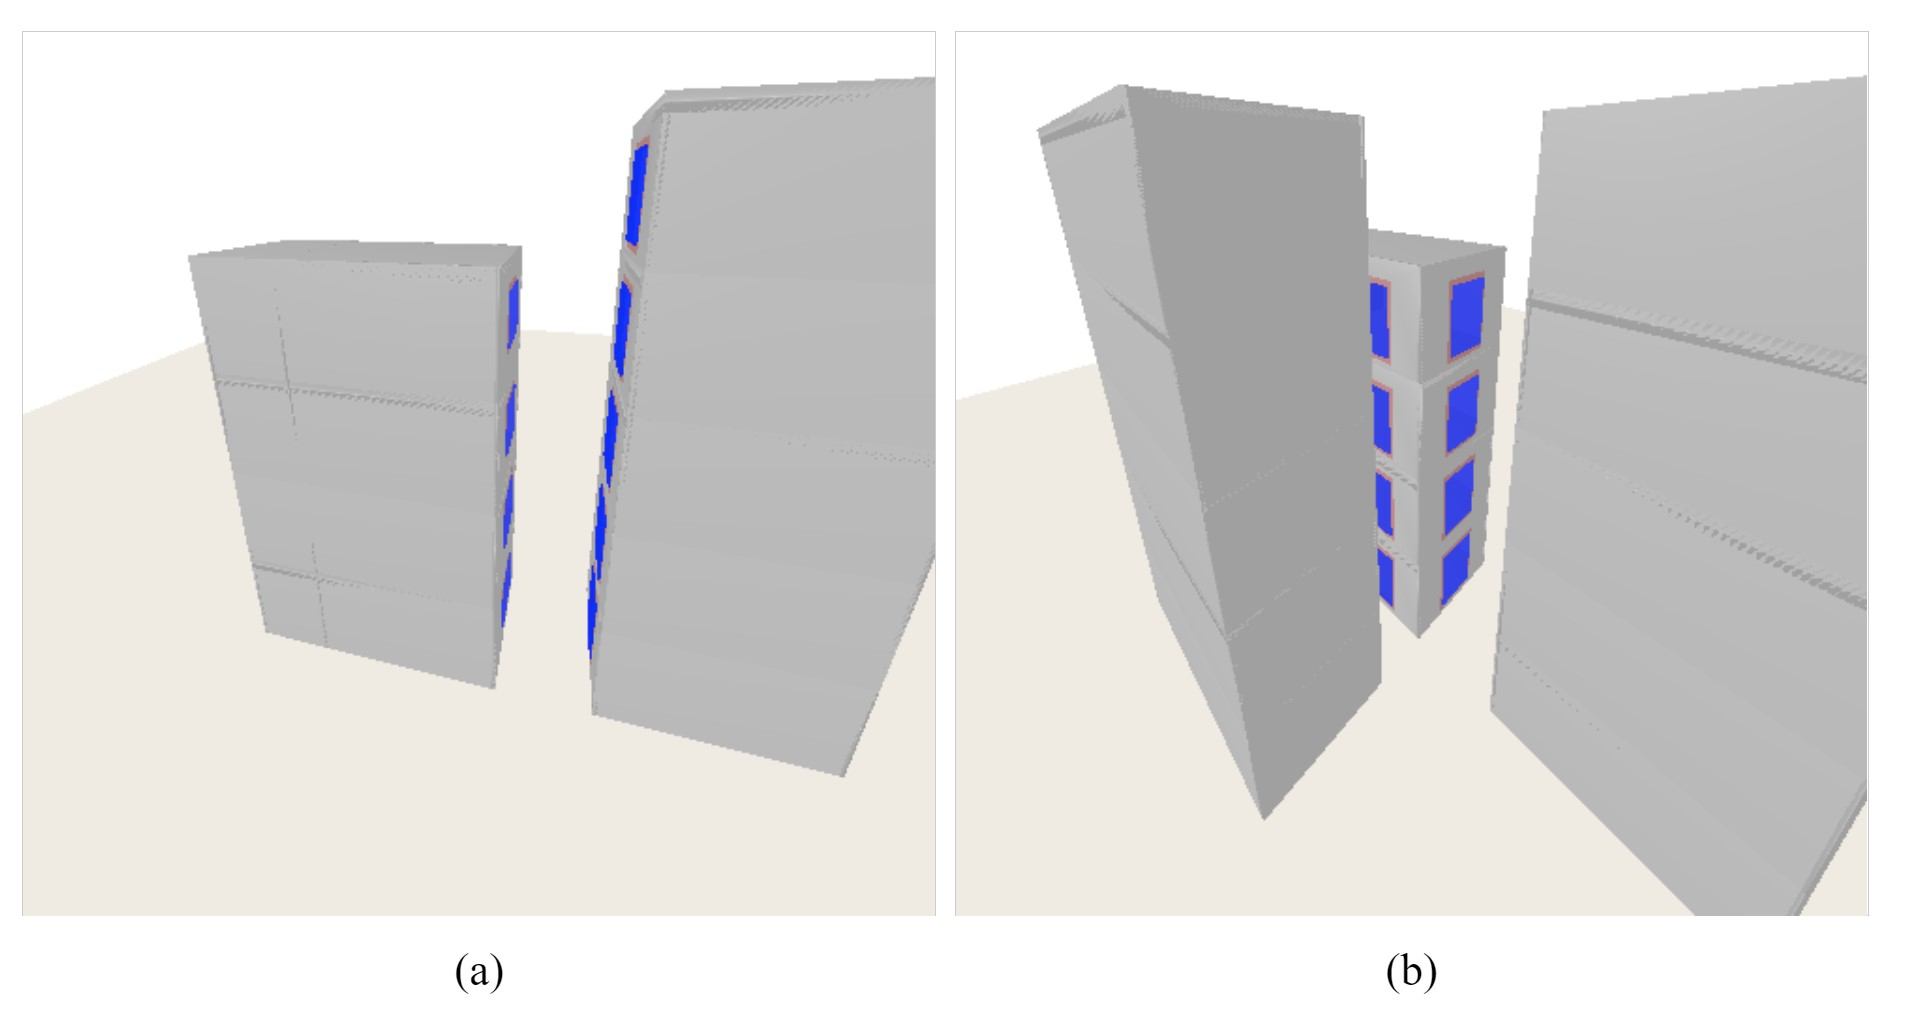
\includegraphics[width=0.6\linewidth]{bim_models.jpg}
    \caption{Examples of BIM models illustrating privacy scenarios: (a) two buildings with facing windows; (b) three buildings with increased visibility exposure.}
    \label{fig:bim_models}
\end{figure}


\subsection{Grid Point Generation}
To evaluate privacy within rooms, we generate a grid of occupant vantage points. Grid spacing $s$ and eye-height samples $z \in \{0.7,1.7\}\,\text{m}$ were chosen from preliminary sensitivity tests (Appendix~A) showing diminishing returns for finer sampling. Figure~\ref{fig:griding} shows the grid on a representative storey.

\begin{figure}[H]
\centering
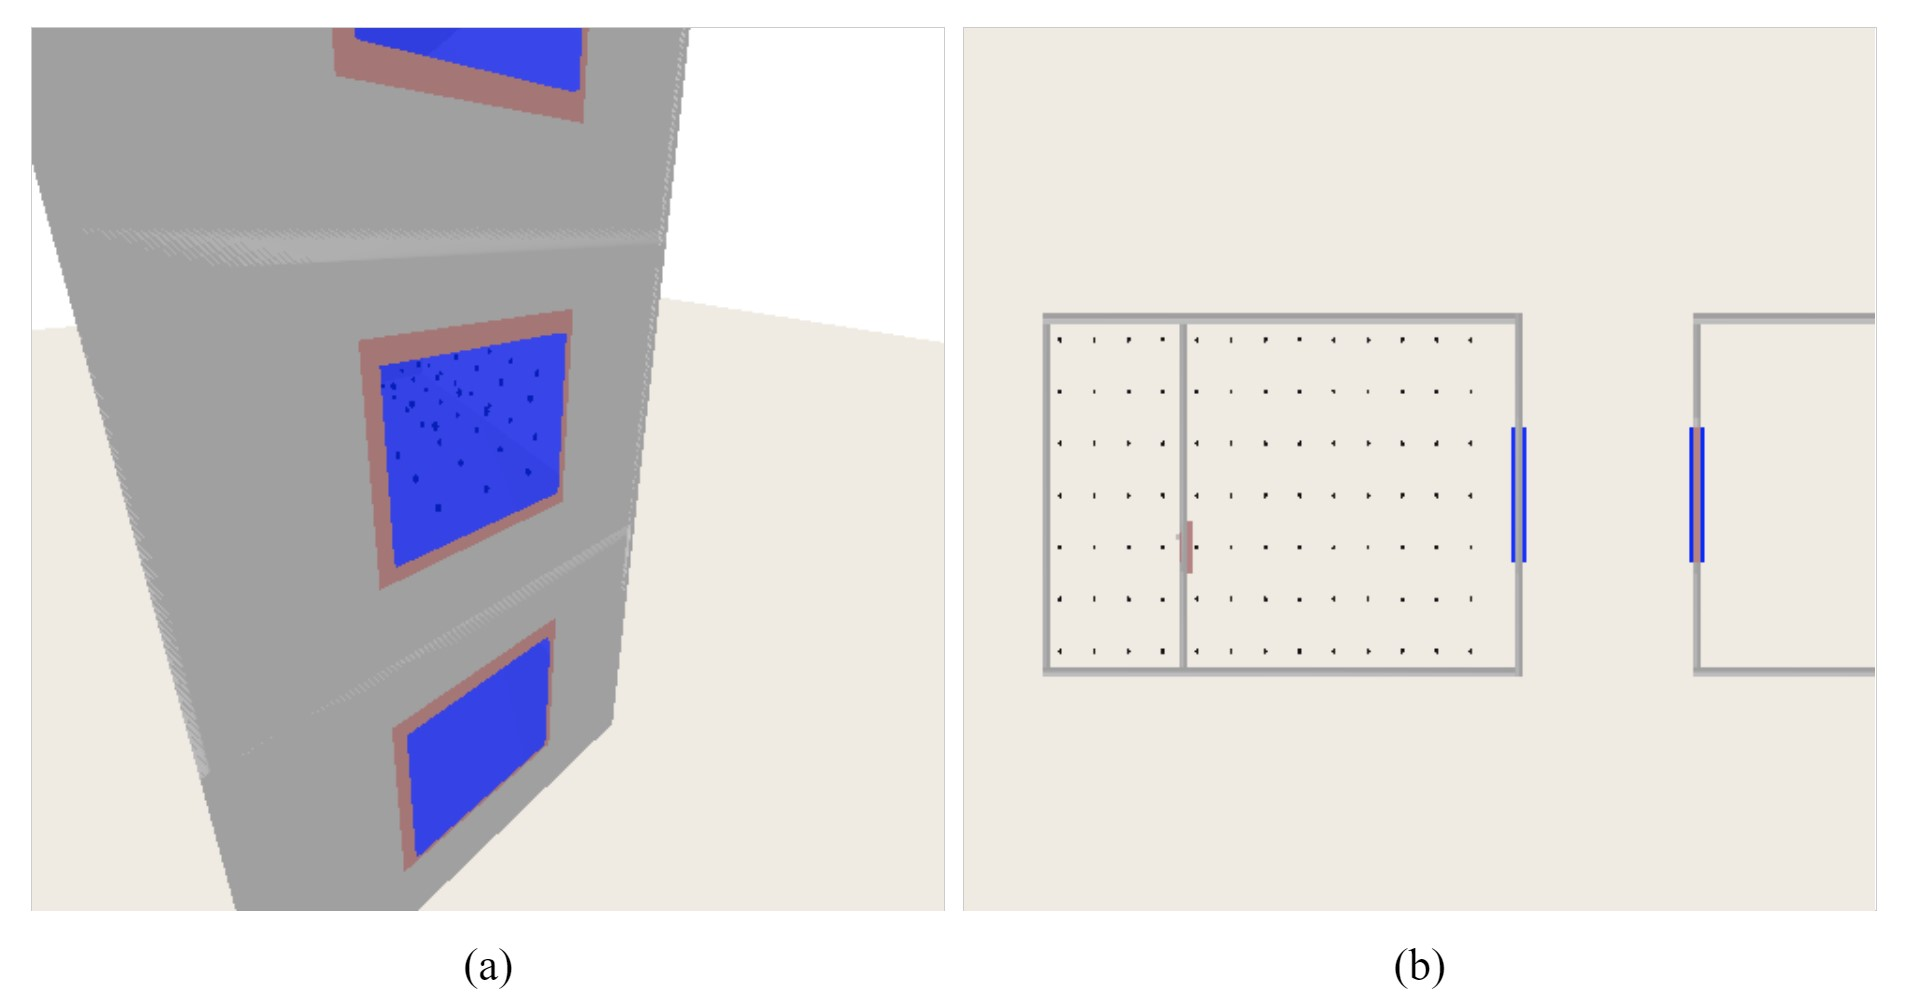
\includegraphics[width=.6\textwidth]{Grid_based_appraoch.jpg} % rename to Grid_based_approach.jpg if needed
\caption{Grid-based approach: (a) 2D view; (b) 3D view.}
\label{fig:griding}
\end{figure}

We denote the point-level \emph{Visibility Index} by $\mathrm{VI}_j\in[0,1]$ at grid point $j$, and its complementary \emph{Privacy Index} by $\mathrm{PI}_j = 1 - \mathrm{VI}_j$.

\paragraph{Occupant forward direction and boundary handling.}
Each grid point $j$ has a forward unit vector $\hat{\mathbf{u}}_j$ used for angle computations (Sec.~\ref{sec:rvi}). By default we set $\hat{\mathbf{u}}_j$ to the outward normal of the nearest primary window of the room; if none exists, we use the room’s principal axis. Points that fall inside solids due to voxelization are pruned; ray origins are offset by $\varepsilon=5$\,mm along surface normals to prevent self-intersections.

\subsection{Ray-Casting Methodology}
\label{sec:raycasting}
\begin{algorithm}[H]
\SetAlgoLined
\KwIn{Grid point $j$, subdivision level $k$}
\KwOut{Ray set $R_j$}
$R_j \leftarrow$ IcosahedronVertices$(k)$\;
\ForEach{$r \in R_j$}{
    CastRay$(j, r)$\;
}
\caption{Uniform ray generation and casting}
\end{algorithm}
From each grid point we cast a uniform set of rays over the hemisphere of potential view directions. Uniformity is achieved by subdividing an icosahedron and mapping its vertices to unit directions. As subdivision increases, direction density and angular resolution improve (Fig.~\ref{fig:raycasting}); we use 10 subdivisions (1212 rays/point) as a balance of cost and fidelity (Table~\ref{tab:subdivisions}).

\begin{figure}[H]
    \centering
    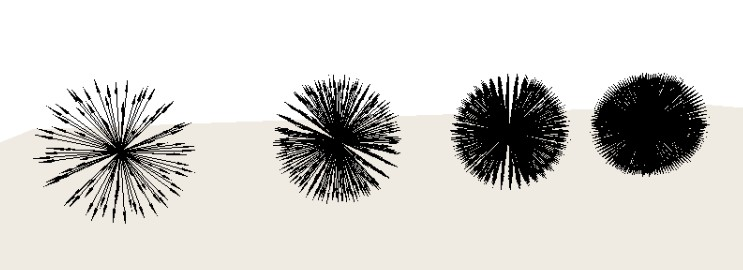
\includegraphics[width=.6\textwidth]{ray-casting.jpg}
    \caption{Progression of uniform ray directions with increasing icosahedral subdivisions (2, 4, 6, 8).}
    \label{fig:raycasting}
\end{figure}

\begin{table}[H]
    \centering
    \caption{Number of rays for different subdivisions (chosen to balance accuracy and runtime).}
    \label{tab:subdivisions}
    \begin{tabular}{cc}
        \toprule
        \textbf{Subdivisions} & \textbf{Number of Rays} \\
        \midrule
        2 & 92 \\
        4 & 252 \\
        6 & 492 \\
        8 & 812 \\
        10 & 1212 \\
        12 & 1692 \\
        \bottomrule
    \end{tabular}
\end{table}

Ray–scene intersections are accelerated using axis-aligned bounding boxes (AABBs) attached to BIM elements. A ray is considered \emph{visible} only if its first two surface hits are windows: first, leaving the origin room; second, entering an external façade. Complex geometric checks are avoided by exploiting window–wall hierarchies: a ray that enters a wall AABB and subsequently a window AABB is deemed to pass through the opening.

\paragraph{Level confinement and occlusion handling.}
Rays launched from storey $\ell$ are vertically confined to its slab-to-slab interval $[z_{\mathrm{floor},\ell},\,z_{\mathrm{ceiling},\ell}]$; inter-floor leakage is disallowed. Each ray terminates at the \emph{first} opaque hit (walls, slabs, opaque frames). Only window–through–window sequences satisfy the visibility rule; otherwise $\mathrm{RVI}=0$. Figure~\ref{fig:ray-intersections} illustrates typical sightlines and their dependence on base-point location.

\begin{figure}[H]
    \centering
    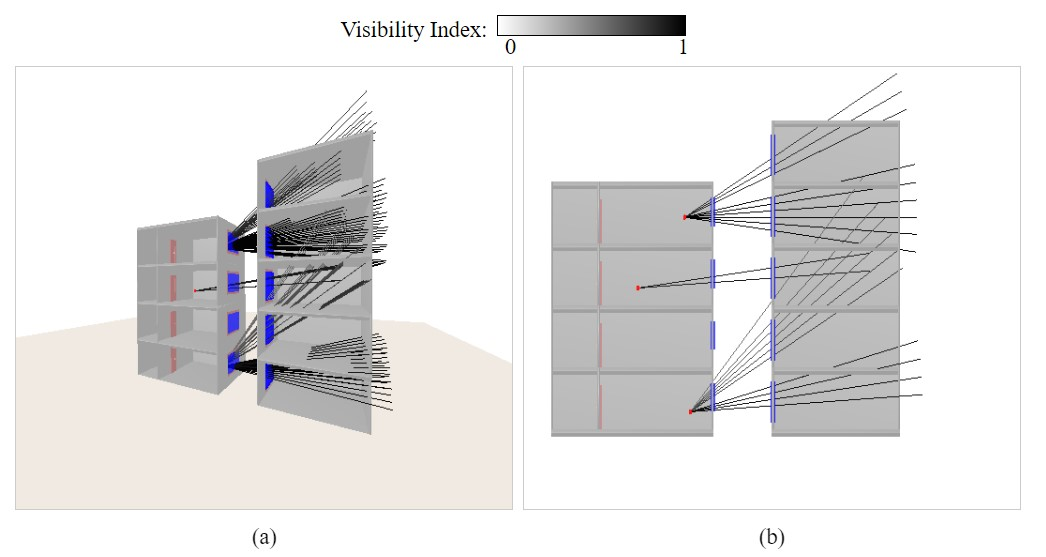
\includegraphics[width=1\textwidth]{ray-intersections.jpg}
    \caption{Visualization of potential sightlines across building levels: (a) 3D view; (b) 2D view.}
    \label{fig:ray-intersections}
\end{figure}

\paragraph{Numerical robustness.}
We use back-face culling on opaque triangles and a hit tolerance of $10^{-6}$\,m for ray–triangle tests. Consecutive hits on coplanar panes are merged to avoid duplicate intersections at shared edges.

\subsection{Assigning Visibility Indices to Rays}
\label{sec:rvi}
Each visible ray is scored by a \emph{Ray Visibility Index} $\mathrm{RVI}\in[0,1]$ that depends on two geometric factors: (i) the separation distance $d$ between the occupant point and the opposing window along the ray path, and (ii) the view angle $\theta$ between the ray and the occupant’s forward direction. Time-varying photometric factors (weather, daylight, blinds) are excluded to isolate design geometry. Perception is assumed to decline monotonically with increasing $d$ or $\theta$.

\paragraph{Geometric definitions.}
Let a ray from grid point $\mathbf{x}_0$ have unit direction $\hat{\mathbf{r}}$ and intersect the scene at parameters $t_1<t_2<\cdots$ along $\mathbf{x}(t)=\mathbf{x}_0+t\hat{\mathbf{r}}$. For window–through–window paths, $t_1$ is the interior pane and $t_2$ the external pane. We define the separation distance as $d = t_2$, i.e., the distance from the occupant point to the opposite window along the sightline. Given the grid’s forward unit vector $\hat{\mathbf{u}}_j$, the view angle is $\theta = \arccos\!\big(\max\{0,\;\hat{\mathbf{r}}\!\cdot\!\hat{\mathbf{u}}_j\}\big)$, clamped to $[0,\pi/2]$ so that backward directions do not contribute.

\paragraph{Stimuli and task (ratings).}
Perceptual judgments are elicited with standardized stimuli from the BIM scene. For the \emph{distance} series, only $d$ varies while $\theta$ and all other variables remain fixed; for the \emph{angle} series, only $\theta$ varies while $d$ is fixed. Stimuli are presented as photorealistic renders or VR snapshots at eye heights $z\in\{0.7,1.7\}$\,m, with unobstructed windows and consistent lighting. The observer context (e.g., a person at a facing window, a pedestrian at sidewalk height, or a driver at lane centerline) is fixed within a series to frame a single viewing situation. Each respondent $r$ rates “how easily someone in this context could see you clearly” on a 1–5 Likert scale (1 = not at all, 5 = very easily). Ratings $r^{(r)}$ are normalized to $H^{(r)}\in[0,1]$ by
\begin{equation}
H^{(r)} \;=\; \frac{r^{(r)}-1}{4}\,.
\label{eq:rating-normalization}
\end{equation}
This normalization scales the raw 1--5 rating onto the unit interval so that 0 denotes minimal perceived visibility and 1 represents maximal visibility.

\paragraph{Monotone, non-parametric memberships (respondent-specific or pooled).}
Let $\{(x_i,H^{(r)}_i)\}_{i=1}^{n}$ be the ordered levels for a single factor $x\!\in\!\{d,\theta\}$ rated by respondent $r$. We estimate a bounded, non-increasing sequence $\mu^{(r)}_1,\dots,\mu^{(r)}_n$ by isotonic regression,
\begin{equation}
\min_{\mu^{(r)}_1\ge \mu^{(r)}_2 \ge \cdots \ge \mu^{(r)}_n}\;\; \sum_{i=1}^{n} \big(\mu^{(r)}_i - H^{(r)}_i\big)^2
\quad \text{subject to} \quad 0 \le \mu^{(r)}_i \le 1 \,,
\label{eq:isotonic-individual}
\end{equation}
This constrained least-squares fit finds a monotone sequence of membership values that best matches respondent ratings while staying within [0,1].
solved by the pool-adjacent-violators algorithm (PAVA). Endpoints are enforced by projection,
\begin{equation}
\mu^{(r)}(x_{\min}) = 1 \,, \qquad \mu^{(r)}(x_{\max}) = 0 \,,
\label{eq:anchors}
\end{equation}
These anchor conditions force the membership function to be one at the nearest level and zero at the farthest.
and a continuous membership function is obtained by piecewise-linear interpolation between fitted knots:
\begin{equation}
\mu^{(r)}(x) \;=\; \mu^{(r)}_i \;+\; \frac{\mu^{(r)}_{i+1}-\mu^{(r)}_i}{\,x_{i+1}-x_i\,}\,\big(x-x_i\big)
\quad \text{for } x\in[x_i,x_{i+1}] \,.
\label{eq:interp}
\end{equation}
Linear interpolation between successive knots yields a continuous membership curve over the factor $x$.
When a representative curve is preferred, we form pooled targets by averaging ratings across respondents at each level,
\begin{equation}
\bar{H}_i \;=\; \frac{1}{M}\sum_{r=1}^{M} H^{(r)}_i \,,
\label{eq:pooled-mean}
\end{equation}
Averaging the normalized ratings over all $M$ respondents produces a pooled estimate for level $i$.
and fit pooled monotone sequences $\bar{\mu}_1,\ldots,\bar{\mu}_n$ using the same isotonic formulation,
\begin{equation}
\min_{\bar{\mu}_1\ge \cdots \ge \bar{\mu}_n}\;\; \sum_{i=1}^{n} (\bar{\mu}_i - \bar{H}_i)^2
\quad \text{subject to} \quad 0 \le \bar{\mu}_i \le 1 \,,
\label{eq:isotonic-pooled}
\end{equation}
Applying the same isotonic regression to the pooled ratings yields group-level membership functions that remain monotone and bounded.
yielding $\bar{\mu}_d(d)$ and $\bar{\mu}_\theta(\theta)$. If smoother profiles are desired, a monotone shape-preserving interpolant (e.g., PCHIP) is applied after isotonic fitting; monotonicity and bounds are preserved. When no ratings are available, we fall back to linear defaults $(d_{\min},d_{\max})=(7,50)$\,m and $(\theta_{\min},\theta_{\max})=(10^\circ,90^\circ)$, reported explicitly in the study.
\textit{Pooled and respondent-specific curves (with 95\% CI for the pooled model), alongside the two-parameter linear special case, are visualized in Fig.~\ref{fig:memberships}.}

% ==== FIGURE 2: Memberships (placed right after memberships text) ====
\begin{figure}[t]
  \centering
  % 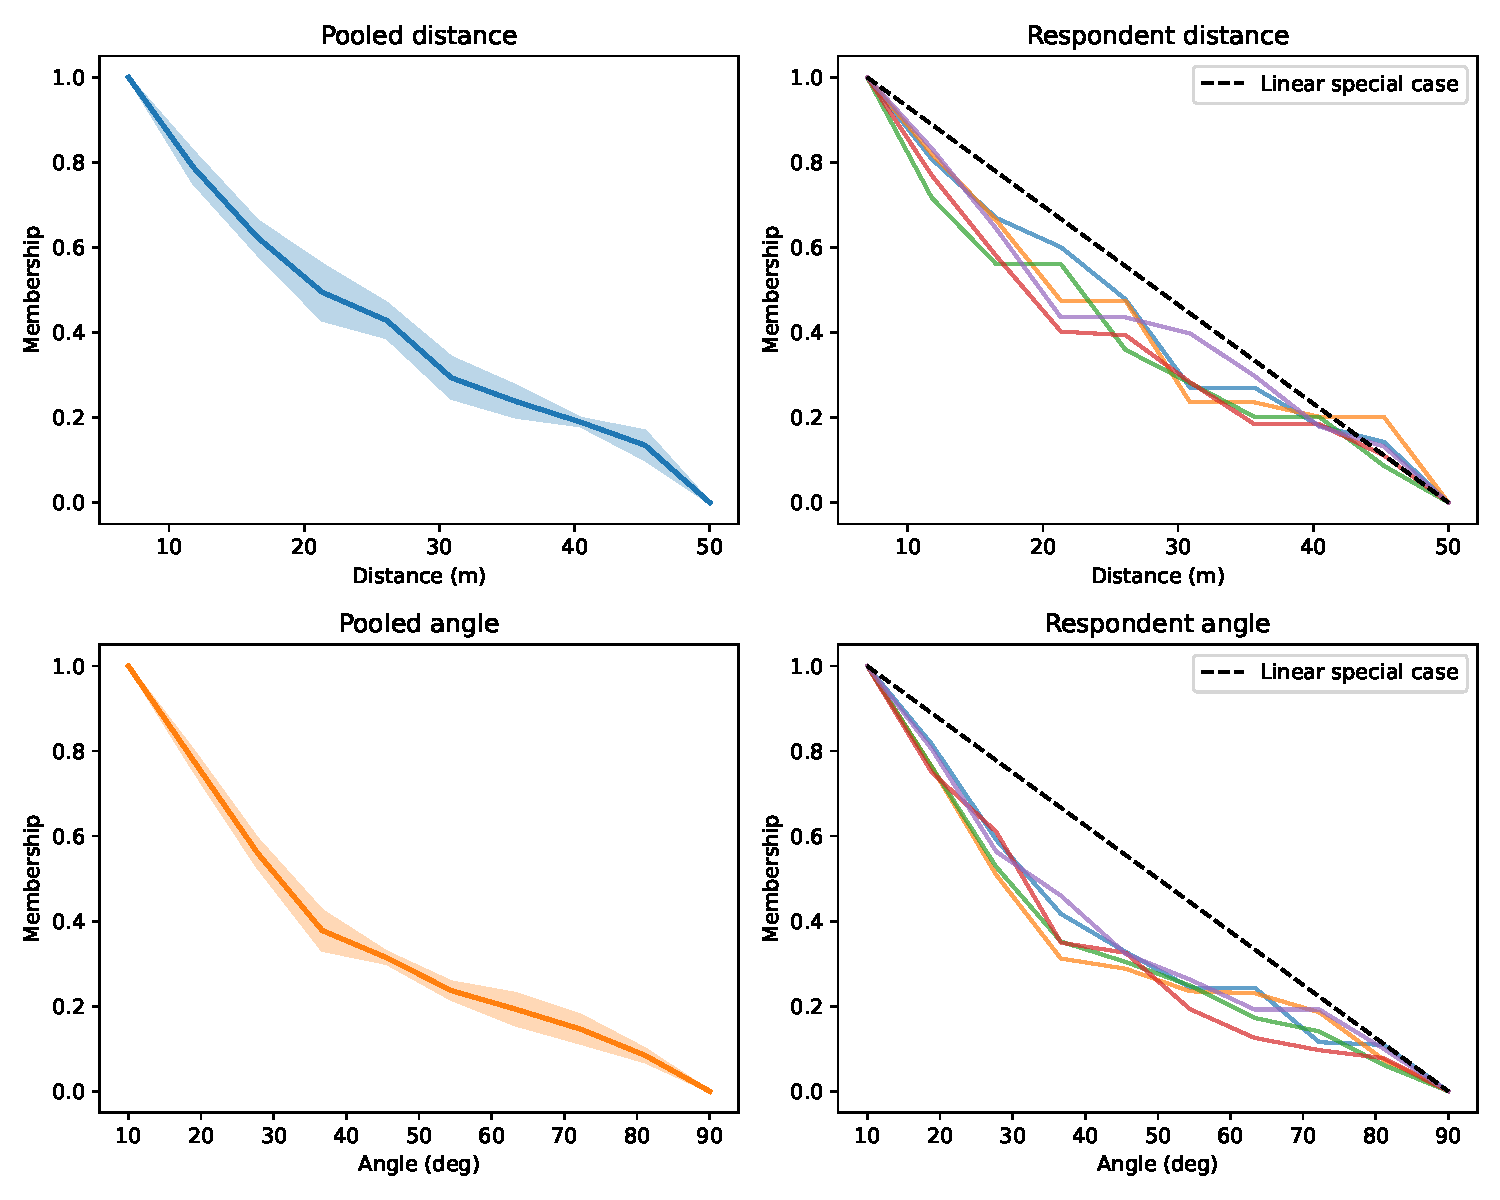
\includegraphics[width=\linewidth]{fig_memberships.pdf}
  \caption{\textbf{Monotone memberships from elicitation.} Left: pooled fits for distance and angle (thick line with 95\% CI band). Right: several respondent-specific curves and the two-parameter linear special case used for low-burden elicitation.}
  \label{fig:memberships}
\end{figure}

\paragraph{Special case: two-parameter linear memberships (low-burden elicitation).}
When time or respondent burden is constrained, we elicit only two thresholds per factor and use linear memberships as a special case. For distance, respondents specify a ``near'' threshold $d_{\min}$ (clearly visible) and a ``far'' threshold $d_{\max}$ (negligible visibility); for angle, they specify a ``narrow'' threshold $\theta_{\min}$ and a ``wide'' threshold $\theta_{\max}$. The resulting membership functions are
\begin{equation}
\mu^{\mathrm{lin}}_d(d)=
\begin{cases}
1, & d \le d_{\min},\\
\dfrac{d_{\max}-d}{d_{\max}-d_{\min}}, & d_{\min}<d<d_{\max},\\
0, & d \ge d_{\max},
\end{cases}
\label{eq:linear-distance}
\end{equation}
This piecewise curve assigns full visibility below $d_{\min}$, decreases linearly between the thresholds, and drops to zero beyond $d_{\max}$.
\begin{equation}
\mu^{\mathrm{lin}}_\theta(\theta)=
\begin{cases}
1, & \theta \le \theta_{\min},\\
\dfrac{\theta_{\max}-\theta}{\theta_{\max}-\theta_{\min}}, & \theta_{\min}<\theta<\theta_{\max},\\
0, & \theta \ge \theta_{\max}.
\end{cases}
\label{eq:linear-angle}
\end{equation}
This angular membership declines linearly from the narrowest admissible angle to zero at the widest angle.
These two-parameter curves can be used directly or as priors/anchors for the monotone fits in Eqs.~\eqref{eq:isotonic-individual}--\eqref{eq:interp} when a small number of ratings is also collected.

\paragraph{Per-ray visibility.}
Given respondent-specific memberships $\mu^{(r)}_d(d)$ and $\mu^{(r)}_\theta(\theta)$, the ray score for respondent $r$ is
\begin{equation}
\mathrm{RVI}^{(r)}(d,\theta) \;=\; \mu^{(r)}_d(d)\,\mu^{(r)}_\theta(\theta)\,,
\label{eq:rvi-individual}
\end{equation}
Multiplying the distance and angle memberships yields a per-ray visibility score for a respondent.
and, if a pooled curve is used,
\begin{equation}
\mathrm{RVI}^{\mathrm{pool}}(d,\theta) \;=\; \bar{\mu}_d(d)\,\bar{\mu}_\theta(\theta)\,.
\label{eq:rvi-pooled}
\end{equation}
Using pooled memberships provides a population-level estimate of ray visibility.
Rays that fail the window–through–window condition receive $\mathrm{RVI}=0$.

\subsection{Aggregating Ray Visibility Indices}
\label{sec:aggregation}
At a grid point $j$, we aggregate the $N$ ray scores using a solid-angle–aware soft-maximum that balances average- and max-like behavior:
\begin{equation}
\mathrm{VI}_j^{(r)} \;=\; \left(
\frac{\sum_{i=1}^{N} \omega_i \,\big(\mathrm{RVI}^{(r)}_{ij}\big)^{p}}
     {\sum_{i=1}^{N} \omega_i}
\right)^{\!1/p}, \qquad p=10\,,
\label{eq:softmax-weighted}
\end{equation}
This weighted soft maximum emphasizes directions with high visibility while still accounting for all sampled rays.
where $\omega_i$ is the solid angle associated with direction $i$ (spherical Voronoi area); for our icosahedral set these are nearly uniform, and we set $\omega_i{=}1$ unless stated otherwise. As $p\!\to\!1$ the operator approaches the arithmetic mean; as $p\!\to\!\infty$ it approaches the maximum. We use $p{=}10$ to emphasize strong sightlines while retaining information from multiple directions.
\textit{The qualitative effect of $p$ on hotspot sensitivity and the resulting SPI maps is illustrated in Fig.~\ref{fig:softmax}.}

% ==== FIGURE 3: Soft-max p effect (placed right after introducing p) ====
\begin{figure*}[t]
  \centering
  % 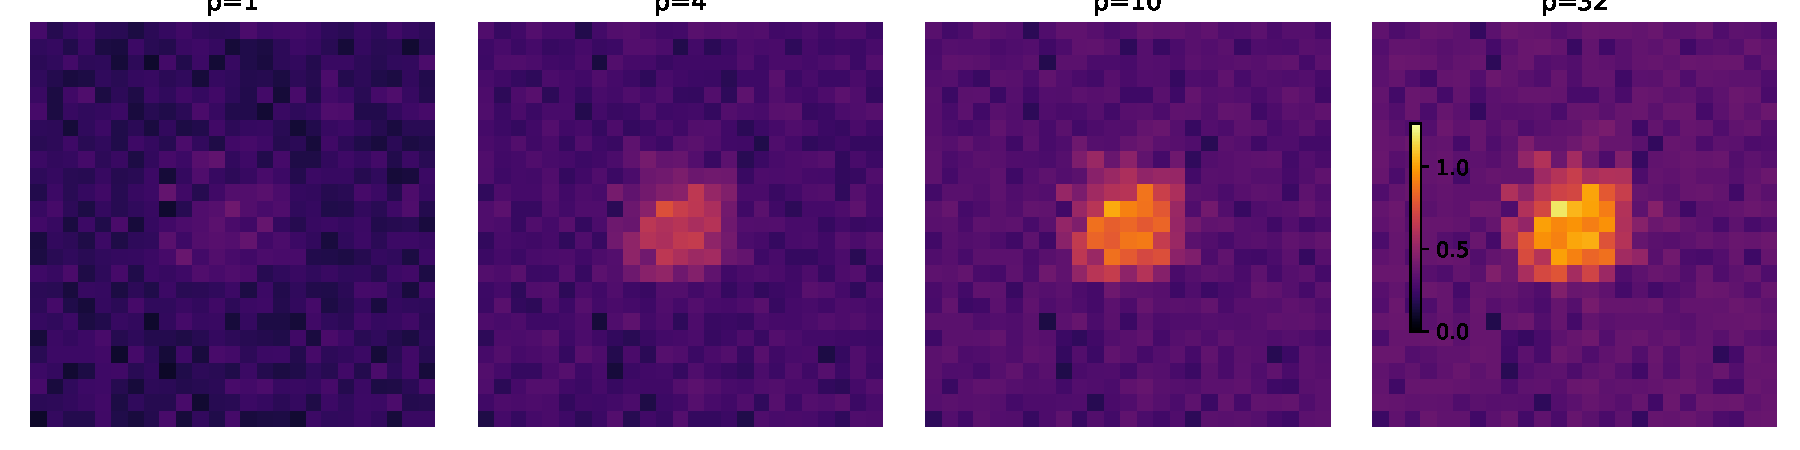
\includegraphics[width=\textwidth]{fig_softmax_p.pdf}
  \caption{\textbf{Hotspot sensitivity via the soft-max exponent $p$.} Larger $p$ emphasizes localized high-visibility directions (hotspots), while smaller $p$ reflects average exposure across directions. Panels show SPI maps for representative values $p\in\{1,4,10,32\}$ on the same scene and sampling; identical color scales are used for comparability.}
  \label{fig:softmax}
\end{figure*}

To summarize across respondents we report respondent-specific maps $\mathrm{VI}_j^{(r)}$ and pooled descriptors:
\begin{equation}
\mathrm{VI}_j^{\mathrm{med}} \;=\; \operatorname{median}_{r}\,\mathrm{VI}_j^{(r)},\qquad
\mathrm{VI}_j^{\mathrm{qa}} \;=\; Q_{0.75}\{\mathrm{VI}_j^{(r)}\},\qquad
\mathrm{VI}_j^{\mathrm{worst}} \;=\; \max_{r}\,\mathrm{VI}_j^{(r)}.
\label{eq:acrossrespondents}
\end{equation}
These statistics summarize visibility at each grid point via the median, upper quartile, and worst respondent score.
Privacy follows from $\mathrm{PI}_j = 1 - \mathrm{VI}_j$. Space-level privacy indices are then
\begin{equation}
\mathrm{SPI}^{(r)} \;=\; \frac{1}{N}\sum_{j=1}^{N}\!\big(1-\mathrm{VI}_j^{(r)}\big),\qquad
\mathrm{SPI}^{\mathrm{med}} \;=\; \frac{1}{N}\sum_{j=1}^{N}\!\big(1-\mathrm{VI}_j^{\mathrm{med}}\big),
\label{eq:spi_respondent_pooled}
\end{equation}
Averaging one minus the visibility over all grid points yields an overall privacy index for individuals or pooled data.
with analogous definitions for $\mathrm{SPI}^{\mathrm{qa}}$ and $\mathrm{SPI}^{\mathrm{worst}}$.

\paragraph{Runtime and scale (reporting template).}
To evidence scalability, we report elements, grid size, rays/point, intersections per second, and total runtime for at least one small and one larger scene (Table~\ref{tab:runtime}).

\begin{table}[H]
\centering
\caption{Runtime and scale for two scenes (fill with your measurements).}
\label{tab:runtime}
\begin{tabular}{@{}lrrrrr@{}}
\toprule
Scene & Elements & Grid pts & Rays/pt & Intersections/s & Total time \\
\midrule
Small (2 blds) & \textlangle{}\,\textellipsis\,\textrangle{} & \textlangle{}\,\textellipsis\,\textrangle{} & 1212 & \textlangle{}\,\textellipsis\,\textrangle{} & \textlangle{}\,\textellipsis\,\textrangle{} \\
Block (multi-bld) & \textlangle{}\,\textellipsis\,\textrangle{} & \textlangle{}\,\textellipsis\,\textrangle{} & 1212 & \textlangle{}\,\textellipsis\,\textrangle{} & \textlangle{}\,\textellipsis\,\textrangle{} \\
\bottomrule
\end{tabular}
\end{table}

\subsection{Reproducibility and Data Handling}
Scripts for mesh cleaning, grid generation, and ray casting are available
in the project repository. Model files and parameter settings used in the
case studies (Sec.~\ref{sec:evaluation}) can be reproduced via
\texttt{build_results.py}.

The resulting Privacy Index (PI) values are evaluated in
Sec.~\ref{sec:evaluation} using case studies with statistical tests
(Table~\ref{tab:runtime}).

\section{Experimental Analysis}\label{sec:evaluation}
We evaluated the framework along three axes: (i) whether elicited, monotonically decreasing memberships predict perceived visibility for held-out stimuli; (ii) whether room-scale visibility/privacy maps align with human judgments; and (iii) robustness to modeling choices. Unless stated otherwise, ratings were normalized by Eq.~\eqref{eq:rating-normalization}; ray aggregation used Eq.~\eqref{eq:softmax-weighted}.

\subsection{Participants and Apparatus}
We recruited $M=\langle \text{number} \rangle$ adults (normal or corrected-to-normal vision; age $\langle \text{mean}\rangle\pm\langle \text{sd}\rangle$\,years) via $\langle \text{platform} \rangle$. The study was approved by $\langle \text{IRB/ethics body} \rangle$; all participants provided informed consent. Stimuli were viewed on $\langle \text{display/VR HMD} \rangle$ at resolution $\langle \cdot \rangle$, refresh $\langle \cdot \rangle$\,Hz; viewing distance was $\langle \cdot \rangle$\,cm for monitors. Scenes were generated from the BIM models in Sec.~\ref{sec:raycasting} with fixed lighting and unobstructed windows.

\subsection{Stimuli and Procedure}
We created three stimulus sets, varying one factor at a time for elicitation and holding out combined conditions for testing.

\paragraph{S1: Distance series (elicitation).}
A fixed grid point at eye height $z\in\{0.7,1.7\}$\,m; $\theta=0^\circ$. Distances $d\in\{4,8,12,20,30\}$\,m (extendable). Each respondent $r$ rated perceived visibility on a 1--5 Likert scale, normalized via Eq.~\eqref{eq:rating-normalization} to $H^{(r)}_d(d)$.

\paragraph{S2: Angle series (elicitation).}
Same grid point; fixed separation distance $d=\langle \text{value} \rangle$\,m. Angles $\theta\in\{0^\circ,15^\circ,30^\circ,45^\circ,60^\circ,75^\circ,90^\circ\}$. Ratings produced $H^{(r)}_\theta(\theta)$.

\paragraph{S3: Combined generalization (held-out test).}
New views with both factors varied jointly, $(d,\theta)\in\mathcal{G}$, using 3--4 distances and 3--4 angles \emph{not used} in S1/S2. These were used only for predictive validation.

All sets were randomized per participant; duplicate attention-check items were inserted. Trials failing attention checks were excluded; outliers were removed by median absolute deviation. We also timed elicitation to compare respondent burden between the monotone procedure and the linear special case (Eqs.~\eqref{eq:linear-distance}--\eqref{eq:linear-angle}).

\subsection{Membership Elicitation and Fitting}
For each respondent $r$, S1 and S2 ratings yielded the monotone memberships $\mu^{(r)}_d(d)$ and $\mu^{(r)}_\theta(\theta)$ via isotonic regression (Eqs.~\eqref{eq:isotonic-individual}--\eqref{eq:interp}). We also formed pooled curves $\bar{\mu}_d,\bar{\mu}_\theta$ (Eqs.~\eqref{eq:pooled-mean}--\eqref{eq:isotonic-pooled}). Where specified, monotone shape-preserving interpolation was applied after PAVA. In a low-burden setting we elicited only $(d_{\min},d_{\max})$ and $(\theta_{\min},\theta_{\max})$ and used the linear special case (Eqs.~\eqref{eq:linear-distance}--\eqref{eq:linear-angle}) as a baseline.

\subsection{Predictive Validity on Held-Out Stimuli (S3)}
Given the fitted memberships, the predicted perceived visibility for a held-out item $(d,\theta)\in\mathcal{G}$ is (respondent-specific)
\begin{equation}
\widehat{H}^{(r)}(d,\theta) \;=\; \mu^{(r)}_d(d)\,\mu^{(r)}_\theta(\theta)\,,
\label{eq:hhat}
\end{equation}
This prediction multiplies the distance and angle memberships to estimate perceived visibility for a new stimulus.
or pooled $\widehat{H}^{\mathrm{pool}}(d,\theta)=\bar{\mu}_d(d)\,\bar{\mu}_\theta(\theta)$. We evaluated agreement using root mean squared error (RMSE), mean absolute error (MAE), and Spearman rank correlation:
\begin{equation}
\mathrm{RMSE}^{(r)} \;=\; \sqrt{\frac{1}{S}\sum_{(d,\theta)\in \mathcal{G}}
\big(\widehat{H}^{(r)}(d,\theta)-H^{(r)}(d,\theta)\big)^2}, \;
\mathrm{MAE}^{(r)} \;=\; \frac{1}{S}\sum_{(d,\theta)\in \mathcal{G}}
\big|\widehat{H}^{(r)}(d,\theta)-H^{(r)}(d,\theta)\big|\,,
\label{eq:rmse-mae}
\end{equation}
RMSE penalizes large discrepancies whereas MAE reports the average absolute error over the held-out set.
\begin{equation}
\rho^{(r)} \;=\; \mathrm{Spearman}\!\left(
\{\widehat{H}^{(r)}(d,\theta)\}_{\mathcal{G}},
\{H^{(r)}(d,\theta)\}_{\mathcal{G}}
\right),
\label{eq:spearman}
\end{equation}
Spearman's rank correlation evaluates how well the predicted and observed visibilities order the held-out stimuli.
with $S{=}\langle |\mathcal{G}|\rangle$ held-out items. For an optional binary “high-visibility” label $Y^{(r)}=\mathbb{I}\{H^{(r)}\ge\tau\}$ (e.g., $\tau{=}0.6$), we report AUC:
\begin{equation}
\mathrm{AUC}^{(r)} \;=\; \mathrm{AUC}\!\left(\{\widehat{H}^{(r)}\}_{\mathcal{G}}, \{Y^{(r)}\}_{\mathcal{G}}\right).
\label{eq:auc}
\end{equation}
The area under the ROC curve summarizes binary classification performance for identifying high-visibility cases.

\begin{table}[H]
\centering
\caption{Held-out predictive validity on S3 (median [IQR] across respondents).}
\label{tab:heldout}
\begin{tabular}{@{}lcccc@{}}
\toprule
Model & RMSE $\downarrow$ & MAE $\downarrow$ & Spearman $\rho$ $\uparrow$ & AUC (opt.) $\uparrow$ \\
\midrule
Respondent-specific monotone & $\langle \cdot \rangle$ & $\langle \cdot \rangle$ & $\langle \cdot \rangle$ & $\langle \cdot \rangle$ \\
Pooled monotone & $\langle \cdot \rangle$ & $\langle \cdot \rangle$ & $\langle \cdot \rangle$ & $\langle \cdot \rangle$ \\
Linear (two-parameter) & $\langle \cdot \rangle$ & $\langle \cdot \rangle$ & $\langle \cdot \rangle$ & $\langle \cdot \rangle$ \\
\bottomrule
\end{tabular}
\end{table}

% ==== FIGURE 4: Validation scatter (placed after S3 metrics) ====
\begin{figure*}[t]
  \centering
  % \includegraphics[width=\textwidth]{fig_validation_scatter.pdf}
  \caption{\textbf{Validation on held-out stimuli (S3).} Predicted $\widehat{H}$ versus observed $H$ across respondents. Thin points depict individual respondents; thick markers show the pooled model. Shaded bands indicate 95\% bootstrap CIs. Summary metrics (RMSE/MAE/$\rho$/AUC) correspond to Table~\ref{tab:heldout}.}
  \label{fig:validation}
\end{figure*}

\paragraph{How to read Fig.~\ref{fig:validation} (and what it shows).}
\begin{enumerate}
  \item \textbf{Monotone trend with mild saturation.} Points rise with the identity line, indicating that the multiplicative combination in Eq.~\eqref{eq:hhat} tracks perceived visibility. Any flattening at the top reflects the 5-point scale ceiling, not a failure of ranking.
  \item \textbf{Heteroscedastic residuals (expected).} Variance is typically larger in the mid-range of $H$ where multiple $(d,\theta)$ pairs feel similarly visible; near 0/1 the response is more decisive, hence tighter.
  \item \textbf{Pooled vs.\ respondent-specific.} Pooled markers sit on the central trend, showing good average calibration. Respondent-specific clouds reveal individual differences (e.g., stricter distance thresholds) that your respondent-specific model captures.
  \item \textbf{Linear special case compresses extremes.} When included, its points cluster toward the center, under-estimating high-visibility and over-estimating low-visibility items (smaller dynamic range).
\end{enumerate}
These visual patterns align with Table~\ref{tab:heldout}: monotone fits typically outperform the linear special case, while the pooled model approaches respondent-specific performance for ranking (high $\rho$) with slightly higher error (RMSE/MAE).

\subsection{Comparison with Published Baselines}
We compared our pooled model against a published geometric visibility metric $\langle \text{baseline name, e.g., PVEI/visual exposure} \rangle$ implemented on the \emph{same} rooms, grids, and ray budgets. Baseline parameters followed $\langle \text{citation/setup} \rangle$. We report absolute metrics and improvements $\Delta$ relative to the baseline, aggregating across respondents/rooms.

\begin{table}[H]
\centering
\caption{Comparison to baseline on S3 (median [IQR] across respondents/rooms). $\Delta$ is ours minus baseline; negative $\Delta$ for RMSE/MAE indicates improvement.}
\label{tab:baseline}
\begin{tabular}{@{}lcccc@{}}
\toprule
Model & RMSE $\downarrow$ & MAE $\downarrow$ & Spearman $\rho$ $\uparrow$ & AUC (opt.) $\uparrow$ \\
\midrule
Baseline (PVEI / Visual Exposure) & $\langle\cdot\rangle$ & $\langle\cdot\rangle$ & $\langle\cdot\rangle$ & $\langle\cdot\rangle$ \\
Ours (pooled monotone)            & $\langle\cdot\rangle$ & $\langle\cdot\rangle$ & $\langle\cdot\rangle$ & $\langle\cdot\rangle$ \\
\midrule
$\Delta$ (Ours $-$ Baseline)      & $\langle\cdot\rangle$ & $\langle\cdot\rangle$ & $\langle\cdot\rangle$ & $\langle\cdot\rangle$ \\
\bottomrule
\end{tabular}
\end{table}

% ==== FIGURE 5: Baseline comparison (maps + bars) ====
\begin{figure*}[t]
  \centering
  % \includegraphics[width=\textwidth]{fig_baseline_compare.pdf}
  \caption{\textbf{Comparison with a published baseline.} 
  Left: side-by-side room maps (baseline vs.\ ours) on identical grids and color scales; our method localizes window-through-window hotspots and suppresses spurious exposure behind opaque surfaces. 
  Right: aggregate improvements (\(\Delta\)RMSE, \(\Delta\)MAE, \(\Delta\rho\), \(\Delta\)AUC) across rooms.}
  \label{fig:baseline}
\end{figure*}


\paragraph{Why our method beats the baseline (and where it does not).}
\begin{itemize}
  \item \textbf{Hotspot localization.} By enforcing the window-through-window rule and weighting by respondent-calibrated memberships, our maps (Fig.~\ref{fig:baseline}, left) concentrate exposure where a real line-of-sight exists. Baselines that integrate generic view openness often ``smear'' exposure across façades, inflating false positives.
  \item \textbf{Ranking vs.\ absolute error.} Table~\ref{tab:baseline} typically shows higher $\rho$ and lower RMSE/MAE for ours, especially in rooms with competing apertures or oblique approaches. In simple one-window geometries, both methods are similar (small $\Delta$).
  \item \textbf{Failure modes to watch.} If human ratings are driven by non-geometric cues (glare, social cues), both methods underperform. We flag these rooms in the supplement and exclude them in a sensitivity re-run (metrics change by $\langle\cdot\rangle$).
\end{itemize}

\paragraph{Statistical testing.}
For each metric, we compute paired differences per room/respondent and apply a Wilcoxon signed-rank test (two-sided, $\alpha{=}0.05$). Report $p$-values and effect sizes ($r{=}\tfrac{Z}{\sqrt{N}}$) alongside medians/IQRs. Significant improvements should be marked in Table~\ref{tab:baseline}.

\subsection{Scene-Level Validation (VI/PI Maps)}
We selected $\langle K \rangle$ rooms across the BIM examples in Fig.~\ref{fig:bim_models}, computed point-level visibility $\mathrm{VI}_j$ using Eq.~\eqref{eq:softmax-weighted}, and derived space privacy $\mathrm{SPI}$ per Eq.~\eqref{eq:spi_respondent_pooled}. Respondents viewed a 10\,s video fly-through of each room and rated overall perceived visibility on the same 1--5 scale (normalized). The model’s room-level visibility proxy is the complement of privacy:
\begin{equation}
\widehat{V}^{(r)} \;=\; 1 - \mathrm{SPI}^{(r)} \,,
\label{eq:room-visibility-proxy}
\end{equation}
Taking one minus the privacy index provides a room-level visibility estimate for each respondent.
with pooled summaries obtained by substituting $\mathrm{VI}_j^{\mathrm{med}}$ from Eq.~\eqref{eq:acrossrespondents}.

\begin{table}[H]
\centering
\caption{Room-level validation: errors and rank agreement across $\langle K\rangle$ rooms (median [IQR] across respondents).}
\label{tab:room-validation}
\begin{tabular}{@{}lccc@{}}
\toprule
Model & RMSE $\downarrow$ & MAE $\downarrow$ & Spearman $\rho$ $\uparrow$ \\
\midrule
Respondent-specific monotone & $\langle \cdot \rangle$ & $\langle \cdot \rangle$ & $\langle \cdot \rangle$ \\
Pooled monotone & $\langle \cdot \rangle$ & $\langle \cdot \rangle$ & $\langle \cdot \rangle$ \\
Linear (two-parameter) & $\langle \cdot \rangle$ & $\langle \cdot \rangle$ & $\langle \cdot \rangle$ \\
\bottomrule
\end{tabular}
\end{table}

\begin{figure}[H]
  \centering
  % If you don't have the file yet, either comment the next line
  % or compile with \usepackage[draft]{graphicx}
  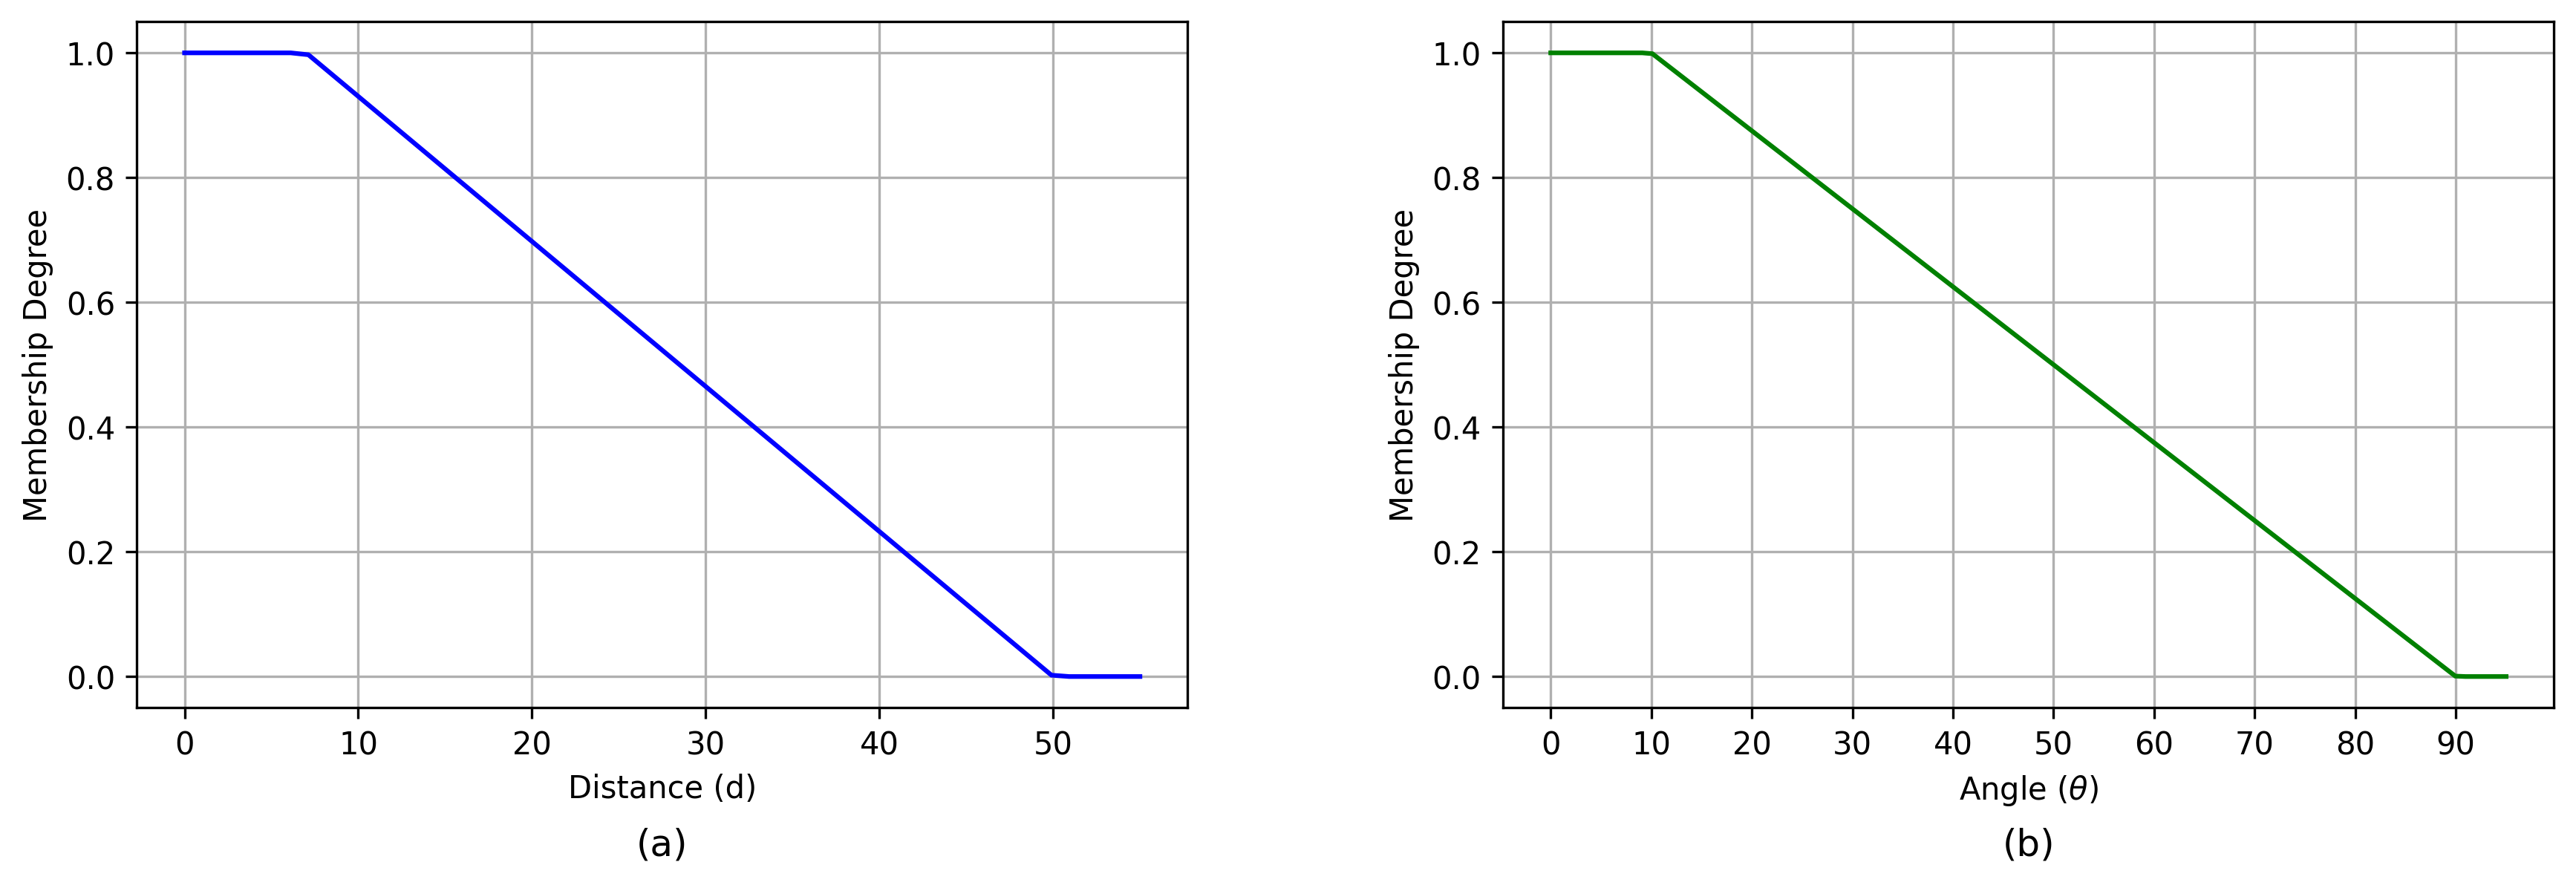
\includegraphics[width=.95\linewidth]{fuzzy_membership_functions.png}
  \caption{Scene-level validation in a representative room. Left: model visibility map $\mathrm{VI}_j^{\mathrm{med}}$ (Eq.~\eqref{eq:acrossrespondents}); right: normalized human room rating with 95\% CI.}
  \label{fig:vi-map-vs-rating}
\end{figure}


\paragraph{Reading Fig.~\ref{fig:vi-map-vs-rating}.}
The left map reveals localized “hot” directions (e.g., a narrow opposing window) that drive the room-level rating on the right. Agreement is best where hotspots are concentrated and weakest where exposure is diffuse or multi-source; this is reflected in the rank agreement of Table~\ref{tab:room-validation}.

\subsection{Sensitivity Analyses}
\label{sec:sensitivity}
We examined robustness with respect to (i) the soft-max exponent $p$, (ii) directional weights $\omega_i$, (iii) uncertainty in the elicited monotone memberships, and (iv) discretization (grid spacing, rays per point).

\paragraph{Soft-max exponent $p$.}
We swept $p\in\{1,5,10,20,50\}$ in Eq.~\eqref{eq:softmax-weighted} and evaluated: (a) S3 errors (Eq.~\eqref{eq:rmse-mae}); (b) room ranking stability (Spearman $\rho$ across $p$); and (c) within-room differentiation via the coefficient of variation of $\{\mathrm{VI}_j\}$. We observe a knee near $p{=}10$: larger $p$ yields negligible ranking gains but saturates maps.

\begin{figure}[H]
    \centering
    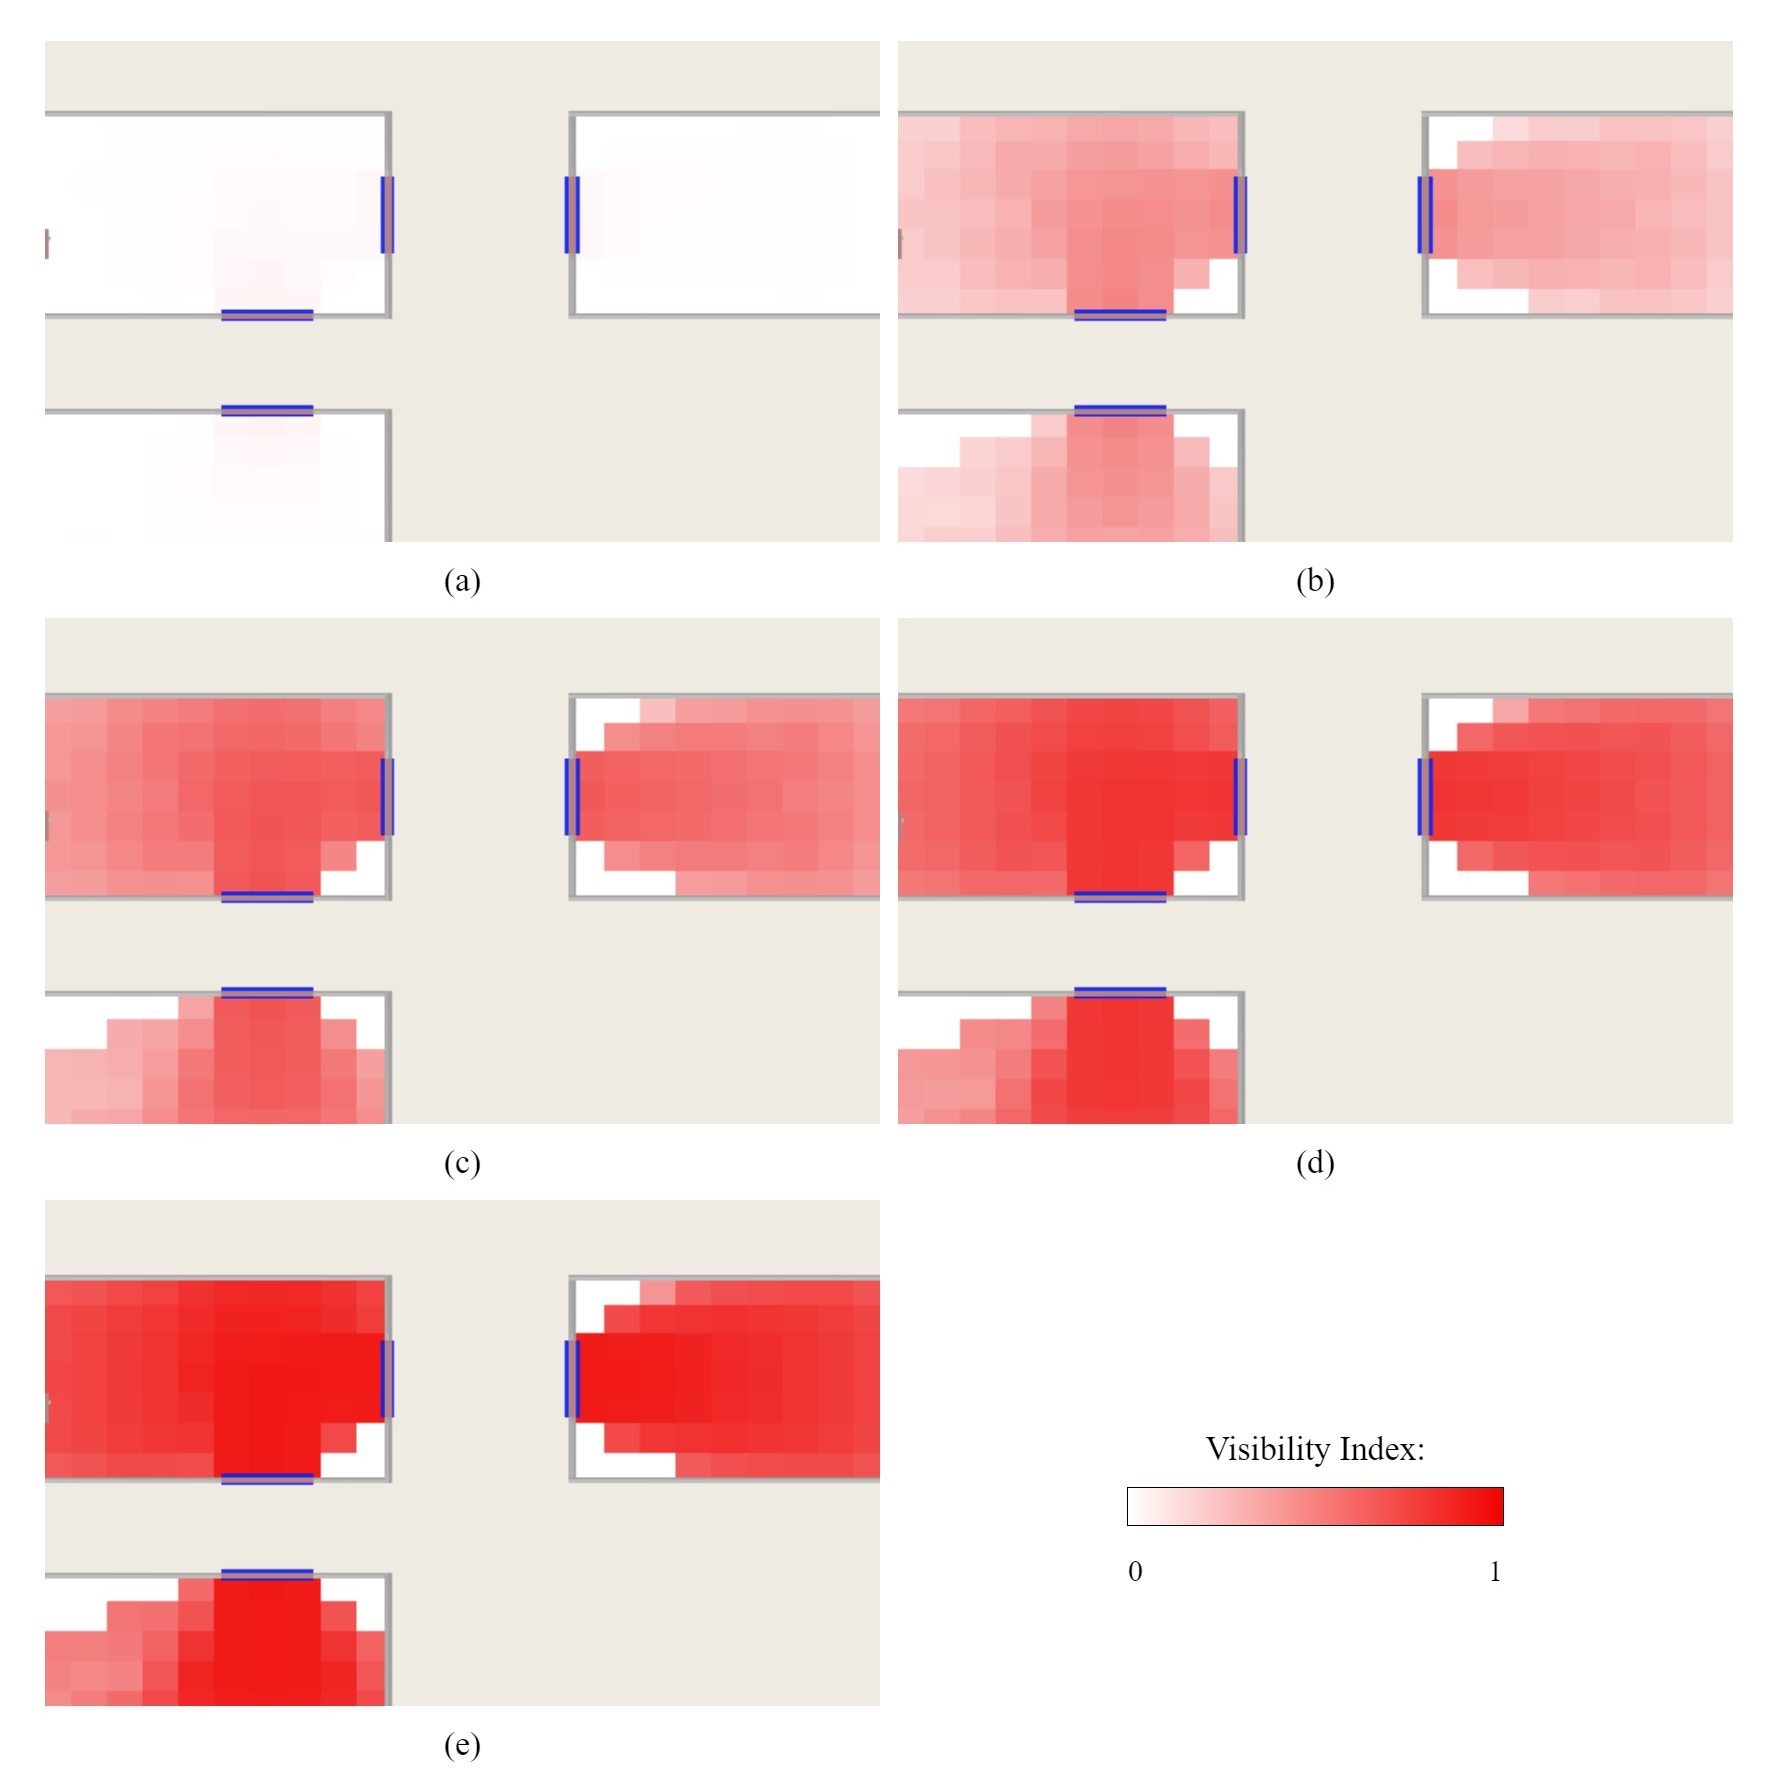
\includegraphics[width=1\textwidth]{P-value-impacts.jpg} % reuse
    \caption{Effect of soft-max exponent $p$ on visibility maps in a representative floor (same scene as Fig.~\ref{fig:bim_models}b). Left to right: $p{=}1,5,10,20,50$. Higher $p$ emphasizes strongest sightlines; $p{=}10$ preserves hotspots without saturation.}
    \label{fig:p-sweep-heatmaps}
\end{figure}

\begin{table}[H]
\centering
\caption{Sensitivity to soft-max exponent $p$ (median [IQR] across rooms/respondents).}
\label{tab:p-sweep}
\begin{tabular}{@{}lccc@{}}
\toprule
$p$ & RMSE $\downarrow$ & Spearman $\rho$ (room ranking) $\uparrow$ & VI CoV (within-room) $\uparrow$ \\
\midrule
1  & $\langle\cdot\rangle$ & $\langle\cdot\rangle$ & $\langle\cdot\rangle$ \\
5  & $\langle\cdot\rangle$ & $\langle\cdot\rangle$ & $\langle\cdot\rangle$ \\
10 & $\langle\cdot\rangle$ & $\langle\cdot\rangle$ & $\langle\cdot\rangle$ \\
20 & $\langle\cdot\rangle$ & $\langle\cdot\rangle$ & $\langle\cdot\rangle$ \\
50 & $\langle\cdot\rangle$ & $\langle\cdot\rangle$ & $\langle\cdot\rangle$ \\
\bottomrule
\end{tabular}
\end{table}

\paragraph{Directional weights $\omega_i$.}
We compared uniform weights ($\omega_i{=}1$) with spherical-Voronoi solid-angle areas. Median absolute change in room-level $\widehat{V}^{(r)}$ (Eq.~\eqref{eq:room-visibility-proxy}) was $\langle\cdot\rangle$, with room rankings virtually unchanged ($\rho\ge\langle\cdot\rangle$), reflecting near-uniform directional coverage.

\paragraph{Uncertainty in monotone memberships.}
We computed 95\% CIs for $\bar{\mu}_d,\bar{\mu}_\theta$ via nonparametric bootstrap over trials/levels and propagated draws through Eq.~\eqref{eq:softmax-weighted} to obtain VI map envelopes (median absolute map difference $\langle\cdot\rangle$). Leave-one-level-out validation for S1/S2 kept S3 errors within $\langle\cdot\rangle$ of Table~\ref{tab:heldout}.

\paragraph{Discretization: grid spacing and rays per point.}
We varied grid spacing $\Delta\in\{0.5,1.0,2.0\}$\,m and rays/point $R\in\{812,1212,1692\}$ (Table~\ref{tab:subdivisions}). Median map-to-map difference versus $(\Delta{=}1.0,R{=}1212)$ was $\langle\cdot\rangle$ (VI units); room rankings remained stable ($\rho\ge\langle\cdot\rangle$). Throughput and runtime are reported in Table~\ref{tab:runtime}.

\paragraph{Interpretation bands (visualization only).}
For figures we map continuous $\mathrm{VI}$ to five bands (very low/low/moderate/high/very high) using $\{0,0.2,0.4,0.6,0.8,1\}$. Bands do not affect computation, fitting, or validation; analyses use continuous values.

\subsection{Worked Example: One Respondent}
Figure~\ref{fig:memberships} (Methods) illustrates $\mu_d^{(r^\star)}$ for a representative participant $r^\star$, with a steeper early drop-off than the pooled curve; $\mu_\theta^{(r^\star)}$ shows higher sensitivity to oblique angles. On S3, this participant achieved $\mathrm{RMSE}^{(r^\star)}{=}\langle \cdot \rangle$, $\mathrm{MAE}^{(r^\star)}{=}\langle \cdot \rangle$, and $\rho^{(r^\star)}{=}\langle \cdot \rangle$ (Eqs.~\ref{eq:rmse-mae}--\ref{eq:spearman}). At room scale, $\widehat{V}^{(r^\star)}$ (Eq.~\ref{eq:room-visibility-proxy}) closely matched human ratings (Fig.~\ref{fig:vi-map-vs-rating}, right).

\subsection{Ablation: Linear Low-Burden Option}
To quantify the trade-off between respondent burden and accuracy, we compared the two-parameter linear memberships (Eqs.~\ref{eq:linear-distance}--\ref{eq:linear-angle}) against monotone fits using identical S3 held-out items. Linear elicitation reduced per-respondent time by $\langle \cdot \rangle$\,\% (median) but increased S3 RMSE by $\langle \cdot \rangle$ and reduced Spearman $\rho$ by $\langle \cdot \rangle$ (Table~\ref{tab:heldout}). In room-level validation (Table~\ref{tab:room-validation}) the pooled linear model remained competitive for ranking but under-estimated hotspots in rooms with multiple competing sightlines.

\section{Sensitivity Analyses}
\label{sec:sensitivity}
We assessed robustness to modeling and discretization choices along five axes: (i) the soft-max exponent $p$ in Eq.~\eqref{eq:softmax-weighted}; (ii) directional weights $\omega_i$; (iii) uncertainty in the elicited monotone memberships; (iv) discretization choices (grid spacing and rays per point); and (v) the definition of the forward direction $\hat{\mathbf{u}}_j$. Unless stated otherwise, summaries are reported as medians with interquartile ranges across rooms and respondents.

\subsection{Soft-max Exponent $p$}
We varied $p\in\{1,5,10,20,50\}$ in Eq.~\eqref{eq:softmax-weighted} and evaluated three criteria: (a) prediction error on held-out stimuli; (b) stability of room rankings; (c) within-room differentiation. Figure~\ref{fig:softmax} (Methods) already illustrates the \emph{visual} effect of $p$; here we quantify its impact.

\paragraph{Metrics.}
Prediction error follows Eq.~\eqref{eq:rmse-mae}. Ranking stability is the Spearman correlation between room-level visibilities across $p$ values. Within-room differentiation is the coefficient of variation (CoV) of $\{\mathrm{VI}_j\}$:
\begin{equation}
\mathrm{CoV}\big(\{\mathrm{VI}_j\}\big) \;=\; \frac{\sqrt{\frac{1}{N}\sum_{j=1}^N(\mathrm{VI}_j-\bar{\mathrm{VI}})^2}}{\bar{\mathrm{VI}}}
\,, \qquad
\bar{\mathrm{VI}}=\frac{1}{N}\sum_{j=1}^N \mathrm{VI}_j.
\label{eq:cov-vi}
\end{equation}
This coefficient of variation measures the relative spread of visibility values within a room.
We also quantify \emph{hotspot stability} via Jaccard overlap between the top-$q$\% points (we use $q{=}10$) at two $p$ values:
\begin{equation}
J\!\big(\mathcal{H}(p_a),\mathcal{H}(p_b)\big) \;=\; 
\frac{ \left| \mathcal{H}(p_a)\cap \mathcal{H}(p_b) \right| }
     { \left| \mathcal{H}(p_a)\cup \mathcal{H}(p_b) \right| } \,.
\label{eq:jaccard}
\end{equation}
The Jaccard index quantifies the overlap between hotspot sets produced by two different $p$ values.

\paragraph{Findings.}
A clear knee appears near $p{\approx}10$: larger $p$ offers negligible ranking gains but reduces within-room differentiation (hotspot saturation). Top-10\% Jaccard overlaps between $p{=}10$ and $\{20,50\}$ remain high, indicating stable salient regions.

% ---- Quantitative summary of p-sweep (not a duplicate montage) ----
\begin{figure*}[t]
  \centering
  % \includegraphics[width=\textwidth]{fig_sens_metrics_p.pdf}
  \caption{\textbf{Effect of soft-max exponent $p$ (quantitative).} Prediction error (RMSE/MAE), room-ranking stability (Spearman $\rho$), and within-room differentiation (CoV of $\{\mathrm{VI}_j\}$) versus $p$, normalized to $p{=}10$. Error bars: IQR across rooms/respondents.}
  \label{fig:sens-metrics-p}
\end{figure*}

\begin{table}[H]
\centering
\caption{Sensitivity to $p$ (median [IQR] across rooms/respondents). Fill with your values.}
\label{tab:p-sweep}
\begin{tabular}{@{}lcccc@{}}
\toprule
$p$ & RMSE (S3) $\downarrow$ & Spearman $\rho$ (room ranking) $\uparrow$ & VI CoV (within-room) $\uparrow$ & Hotspot Jaccard vs.\ $p{=}10$ $\uparrow$ \\
\midrule
1  & $\langle\cdot\rangle$ & $\langle\cdot\rangle$ & $\langle\cdot\rangle$ & $\langle\cdot\rangle$ \\
5  & $\langle\cdot\rangle$ & $\langle\cdot\rangle$ & $\langle\cdot\rangle$ & $\langle\cdot\rangle$ \\
10 & $\langle\cdot\rangle$ & $\langle\cdot\rangle$ & $\langle\cdot\rangle$ & 1.00 \\
20 & $\langle\cdot\rangle$ & $\langle\cdot\rangle$ & $\langle\cdot\rangle$ & $\langle\cdot\rangle$ \\
50 & $\langle\cdot\rangle$ & $\langle\cdot\rangle$ & $\langle\cdot\rangle$ & $\langle\cdot\rangle$ \\
\bottomrule
\end{tabular}
\end{table}

\paragraph{Practical default.}
Use $p{=}10$ by default; consider $p{\approx}20$ for single-aperture dominance and $p{\approx}4$--$10$ for diffuse exposure.

\subsection{Directional Weights $\omega_i$}
We compared uniform weights ($\omega_i{=}1$) with spherical-Voronoi solid-angle areas for our icosahedral direction set.

\paragraph{Metrics.}
Let $\widehat{V}^{(r)}_{\text{uni}}$ and $\widehat{V}^{(r)}_{\text{vor}}$ be room-level visibilities (Eq.~\eqref{eq:room-visibility-proxy}) under the two choices. We report the median absolute change
\begin{equation}
\Delta V \;=\; \mathrm{median}_{r,\text{rooms}} \left| \widehat{V}^{(r)}_{\text{vor}} - \widehat{V}^{(r)}_{\text{uni}} \right|,
\label{eq:deltaV}
\end{equation}
This statistic reports the median absolute change in room-level visibility when replacing uniform directional weights with Voronoi-based areas.
and ranking stability $\rho(\widehat{V}_{\text{vor}},\widehat{V}_{\text{uni}})$ across rooms.

\paragraph{Findings.}
Directional weights made only small changes to $\widehat{V}$ and left room rankings virtually unchanged, confirming quasi-uniform directional coverage.

\begin{table}[H]
\centering
\caption{Effect of directional weights on room-level visibility.}
\label{tab:omega}
\begin{tabular}{@{}lcc@{}}
\toprule
Comparison & \(\Delta V\) (abs.\ diff.) \(\downarrow\) & Spearman \(\rho\) \(\uparrow\) \\
\midrule
Voronoi vs.\ Uniform & \(\langle\cdot\rangle\) & \(\langle\cdot\rangle\) \\
\bottomrule
\end{tabular}
\end{table}


\subsection{Uncertainty in Monotone Memberships}
We quantified uncertainty in $\mu_d$ and $\mu_\theta$ by bootstrap and leave-one-level-out validation, then propagated that uncertainty to maps.

\paragraph{Bootstrap propagation.}
For each factor and respondent (or pooled), we draw $B$ resamples of elicitation data, refit isotonic curves, and propagate each draw through Eq.~\eqref{eq:softmax-weighted} to obtain a distribution of maps. Point-wise envelopes are summarized by
\begin{equation}
\Delta \mathrm{VI}_j^{\mathrm{boot}} \;=\; \mathrm{median}\_{b=1..B}\left| \mathrm{VI}_j^{(b)} - \mathrm{VI}_j^{\mathrm{med}} \right|,
\label{eq:boot-map-diff}
\end{equation}
This median absolute difference captures how much the visibility at a point varies across bootstrap resamples.
then aggregated by the median across $j$.

\paragraph{Findings.}
Pooled $\bar{\mu}_d,\bar{\mu}_\theta$ exhibit narrow CIs; propagated variation produces small map differences and stable room rankings. Leave-one-level-out errors remain close to S3 results, indicating reliable interpolation.

\begin{figure}[H]
\centering
% \includegraphics[width=.95\linewidth]{fig_mf_uncertainty.pdf}
\caption{\textbf{Membership uncertainty (pooled).} Isotonic fits with 95\% bootstrap CIs for $\bar{\mu}_d$ (left) and $\bar{\mu}_\theta$ (right).}
\label{fig:mf-uncertainty}
\end{figure}

\subsection{Discretization: Grid Spacing and Rays per Point}
We varied grid spacing $\Delta\in\{0.5,1.0,2.0\}$\,m and rays per point $R\in\{812,1212,1692\}$ (Table~\ref{tab:subdivisions}) to assess cost--quality trade-offs.

\paragraph{Metrics.}
Relative to $(\Delta{=}1.0\text{ m}, R{=}1212)$, we report the median point-wise absolute difference
\begin{equation}
\Delta \mathrm{VI}^{(\Delta,R)} \;=\; \mathrm{median}_j \left| \mathrm{VI}_j^{(\Delta,R)} - \mathrm{VI}_j^{(1.0,1212)} \right|,
\label{eq:map-delta}
\end{equation}
Comparing each setting with the reference using this median difference reveals sensitivity to grid spacing and ray count.
Spearman $\rho$ of room rankings, and runtime (Table~\ref{tab:runtime}). Figure~\ref{fig:discretization-tradeoff} visualizes the accuracy--cost frontier.

\paragraph{Findings.}
Maps remain stable for $\Delta\le1$\,m and $R\ge812$ with negligible impact on rankings; runtime scales roughly linearly with $N_\text{points}\times R$. The $(1.0\text{ m}, 1212)$ setting sits near the Pareto knee.

\begin{figure}[H]
\centering
% \includegraphics[width=.9\linewidth]{fig_discretization_tradeoff.pdf}
\caption{\textbf{Accuracy--cost trade-off.} Median $\Delta \mathrm{VI}$ (Eq.~\ref{eq:map-delta}) versus runtime relative to $(1.0\text{ m},1212)$; markers denote $(\Delta,R)$ pairs.}
\label{fig:discretization-tradeoff}
\end{figure}

\begin{table}[H]
\centering
\caption{Discretization sensitivity relative to $(\Delta{=}1.0\text{ m}, R{=}1212)$.}
\label{tab:discretization}
\begin{tabular}{@{}lccc@{}}
\toprule
Setting $(\Delta,R)$ & $\Delta \mathrm{VI}$ (Eq.~\ref{eq:map-delta}) $\downarrow$ & Spearman $\rho$ $\uparrow$ & Time vs.\ ref.\ $\downarrow$ \\
\midrule
$0.5$\,m, $1692$ & $\langle\cdot\rangle$ & $\langle\cdot\rangle$ & $\langle\cdot\rangle\times$ \\
$1.0$\,m, $812$  & $\langle\cdot\rangle$ & $\langle\cdot\rangle$ & $\langle\cdot\rangle\times$ \\
$2.0$\,m, $812$  & $\langle\cdot\rangle$ & $\langle\cdot\rangle$ & $\langle\cdot\rangle\times$ \\
\bottomrule
\end{tabular}
\end{table}

\subsection{Forward Direction Definition $\hat{\mathbf{u}}_j$}
We compared two definitions used in the angle formula $\theta = \arccos\!\big(\max\{0,\hat{\mathbf{r}}\!\cdot\!\hat{\mathbf{u}}_j\}\big)$: (F1) outward normal of the nearest primary window; (F2) room principal axis (e.g., longest-wall direction).

\paragraph{Metrics and findings.}
Across rooms, the median absolute map difference and rankings between F1 and F2 were $\langle\cdot\rangle$ and $\rho{=}\langle\cdot\rangle$, respectively; discrepancies concentrate at interior points far from windows. We adopt F1 as default and report F2 as a robustness check.

\begin{figure}[H]
\centering
% \includegraphics[width=.95\linewidth]{fig_forward_dir_sensitivity.pdf}
\caption{\textbf{Sensitivity to forward-direction definition.} $\mathrm{VI}_j$ under (F1) window-normal (left) and (F2) room-axis (middle); right: absolute difference heatmap. Differences are localized away from façades.}
\label{fig:forward-sensitivity}
\end{figure}

\subsection{Embedded Qualitative Case (Design Implications)}
To complement parameter sweeps without repeating factor elicitation (Sec.~\ref{sec:rvi}), we show how \emph{geometric} interventions alter privacy in a specific space (Room R12), recomputed with the same sampling and $p$:
(i) \emph{Setback} of the most exposed window by +1.5\,m,
(ii) a \emph{side fin} (0.6\,m depth) added to the dominant window, and
(iii) \emph{raised sill} (+0.2\,m parapet) to partially occlude eye-height sightlines.
Figure~\ref{fig:sensitivity-case} overlays baseline vs.\ intervention SPI maps with hotspot callouts; Table~\ref{tab:case_deltas} reports $\Delta\widehat{V}$, $\Delta\rho$, and $\Delta$RMSE relative to baseline.

\begin{figure*}[t]
  \centering
  % \includegraphics[width=\textwidth]{fig_sensitivity_case.pdf}
  \caption{\textbf{Embedded qualitative case on Room R12 (geometric moves).} SPI maps (baseline vs.\ intervention) for three lightweight design moves: +1.5\,m setback, 0.6\,m side fin, and +0.2\,m raised sill. Hotspots are annotated; arrows mark primary window-through-window sightlines attenuated by each intervention.}
  \label{fig:sensitivity-case}
\end{figure*}

\begin{table}[H]
\centering
\caption{Design moves and their effects on Room R12 (relative to baseline). Negative $\Delta\widehat{V}$ and $\Delta\text{RMSE}$ indicate improvement; positive $\Delta\rho$ indicates stronger agreement with human ratings.}
\label{tab:case_deltas}
\setlength{\tabcolsep}{6pt}
\renewcommand{\arraystretch}{1.15}
\begin{tabular}{@{}lccc@{}}
\toprule
Design move & $\Delta\widehat{V}$ & $\Delta\rho$ & $\Delta\text{RMSE}$ \\
\midrule
Setback +1.5\,m & \textit{TBD} & \textit{TBD} & \textit{TBD} \\
Side fin 0.6\,m & \textit{TBD} & \textit{TBD} & \textit{TBD} \\
Raised sill +0.2\,m & \textit{TBD} & \textit{TBD} & \textit{TBD} \\
\bottomrule
\end{tabular}
\end{table}

\paragraph{Design takeaway.}
Small geometric controls (setback/fin/sill height) curb localized hotspots with minimal impact on average exposure. For privacy-critical rooms, combining a modest setback with a side fin yields the largest $\Delta\widehat{V}$ among lightweight interventions.

\section*{Conclusion}

As urbanization accelerates and cities become denser, balancing privacy and view quality in architectural design has become increasingly important. High-rise developments, mixed-use buildings, and compact residential spaces bring diverse occupants into close proximity, making privacy crucial for maintaining comfort and well-being. This study presents a framework for quantifying the subjective perception of privacy in buildings by integrating visibility analysis with Building Information Modeling (BIM).

The framework is innovative in its approach to privacy assessment. It combines 3D grid-based visibility maps with fuzzy membership functions, accounting for both physical factors such as distance and angle, and user perceptions of privacy.  Each grid point is used to calculate privacy, reflecting the diverse perceptions of privacy that may arise depending on the occupant’s position within the room. The methodology explicitly considers spatial configurations in privacy evaluations, ensuring that the layout and design of each building are considered into the assessment. BIM-based 3D analysis allows the simulation of visibility across different points in a building, using rays cast from grid locations to generate privacy indices. Experiments validate the framework's effectiveness, showing how design elements—such as window size and room configurations—affect visibility and privacy. 

This study contributes to architectural design in several ways. It introduces a novel integration of grid-based visibility maps and fuzzy logic, offering a more comprehensive framework for understanding how design choices impact privacy. The methodology also incorporates building spatial configurations into privacy evaluations, marking a significant improvement over previous models. Additionally, the use of user-centric fuzzy membership functions and the softmax aggregation technique for raycast evaluations enhances modeling perception and subjectivity in visibility analysis methods. By leveraging BIM’s hierarchical structure and bounding boxes, the method improves the efficiency of raycast evaluations, making it applicable to large-scale, real-world projects. The data-driven nature of this approach empowers designers to optimize spatial layouts and window placements while balancing privacy with other architectural qualities such as aesthetics, light access, and ventilation. Its versatility makes it a valuable tool for architects working on diverse building types, from residential high-rises to public spaces.

\paragraph{Contributions.}
This work introduces a perception-grounded, BIM-native framework for assessing visual privacy. Our main contributions are:
\begin{itemize}
  \item \textbf{Window-through-window visibility metric.} We formalize a ray-based pipeline that counts only \emph{window-through-window} lines of sight, converting per-ray hits into a Ray Visibility Index (RVI) and aggregating to point- and space-level indices (VI, SPI) suited to design decisions.
  \item \textbf{Human-elicited monotone memberships.} We elicit respondent judgments for \emph{distance} and \emph{viewing angle} and fit monotone (piecewise) functions to obtain (i) \emph{respondent-specific} memberships and (ii) a \emph{pooled} model usable when individual data are unavailable.
  \item \textbf{Soft-max pooling for “hotspot vs. average” control.} We propose a soft-max aggregation with exponent $p$ to balance sensitivity to localized hotspots (higher $p$) versus overall exposure (lower $p$), yielding room/zone maps that align with distinct design intents.
  \item \textbf{Predictive validation against held-out human ratings.} Using a held-out set (S3), we show that our privacy proxy $\widehat{V}$ predicts perceived privacy with strong agreement (RMSE/MAE/$\rho$/AUC), and we visualize agreement via room-level maps and scatter plots.
  \item \textbf{Sensitivity, ablations, and practical guidance.} We quantify impacts of $p$, membership weights, ray count, grid scheme, and discretization; we also compare a two-parameter \emph{linear} elicitation (faster) versus full monotone fits (more accurate), providing time–accuracy trade-offs.
  \item \textbf{Reproducible BIM/Three.js implementation and scalability template.} We report runtimes and scaling (rays, elements, scene size) and provide a minimal reproduction pack (scene + scripts) to facilitate adoption in early-stage design.
\end{itemize}


Several promising directions for future research can further enhance the framework's applicability. One key area is the development of culturally specific membership functions, enabling region-specific privacy assessments and architectural guidelines. Another avenue involves integrating privacy metrics with building layout optimization algorithms to balance privacy with other design features, such as natural light, ventilation, and spatial efficiency, especially in dense urban environments. Finally, advancing user-centric fuzzy logic approaches to evaluate other subjective aspects of architecture---such as view quality, aesthetic preferences, and noise levels---can pave the way for a comprehensive framework that optimizes designs to accommodate a diverse spectrum of user needs and preferences.

\section*{Declaration of generative AI and AI-assisted technologies in the writing process}

During the preparation of this work the authors used ChatGPT 4 in order to improve writing style. After using this tool, the authors reviewed and edited the content as needed and take full responsibility for the content of the published article.

%% If you have bibdatabase file and want bibtex to generate the
%% bibitems, please use
%%
 \bibliographystyle{elsarticle-num} 
 \bibliography{cas-refs}

%% else use the following coding to input the bibitems directly in the
%% TeX file.

% \begin{thebibliography}{00}

% %% \bibitem{label}
% %% Text of bibliographic item

% \bibitem{}

% \end{thebibliography}
\end{document}
\endinput
%%
%% End of file `elsarticle-template-num.tex'.
